\documentclass[12pt, a4paper]{article}
\usepackage{mathrsfs, amsmath,amssymb,amsthm,mathtools,setspace,graphicx,array,tikz,url}
\usepackage{cite}
\usepackage[hidelinks]{hyperref}
\usepackage{fancyhdr}
\usepackage{lastpage} 
\usepackage[top=3cm, left=3cm, right=3cm, bottom=3cm]{geometry}
\usepackage{enumitem}
\usepackage{titlesec}
\usepackage{etoolbox}
\usepackage{amsthm} % Required for theorem environments
\usetikzlibrary{decorations.markings}
\patchcmd{\thebibliography}{\advance\leftmargin\labelsep}{\labelsep=.5em\leftmargin=2.5em\itemindent=0em\advance\leftmargin\labelsep}
\titlespacing*{\section}{0pt}{3em}{2em}
\titleformat{\section}
  {\normalfont\large\bfseries} % format for the whole title
  {\thesection}                % section number format
  {0.5em}                      % spacing between number and title
  {}                           % code before the title text

\setstretch{1.1}

\pagestyle{fancy}
\fancyhf{} % Clear header and footer
\fancyfoot[C]{\footnotesize \thepage\ of \pageref{LastPage}}


\renewcommand{\headrulewidth}{0pt}
\renewcommand{\qedsymbol}{$\blacksquare$}

\newtheoremstyle{spaced}
  {15pt}   % Space above (e.g., 10pt)
  {20pt}   % Space below (e.g., 10pt)
  {\itshape} % Body font (e.g., italic)
  {}       % Indentation of the header
  {\bfseries} % Theorem header font (e.g., bold)
  {.}      % Punctuation after theorem header
  {.5em}   % Space after theorem header
  {}       % Theorem head spec (can be left empty)

\newcommand{\chapter}[1]{%
  \par\vspace{2em}%
  \refstepcounter{section}%
  \begin{center}
    \textit{Chapter \thesection} \\[1.5ex]
    \textbf{#1}
  \end{center}
  \vspace{1em}%
}

\theoremstyle{spaced}
\newtheorem{conjecture}{Conjecture}[section]
\newtheorem{theorem}{Theorem}[section]
\newtheorem{definition}{Definition}[section]
\newtheorem{example}{Example}[section]
\newtheorem{lemma}{Lemma}[section]
\newtheorem{proposition}{Proposition}[section]
\newtheorem{corollary}{Corollary}[section]
\newtheorem{remark}{Remark}[section]
\newtheorem{namedlemma}{Negation Lemma}[section]
\newtheorem{exercise}{}
\newcommand{\setexercise}[1]{\setcounter{exercise}{#1-1}}


\title{Function of One Complex Variable I}
\author{
  John B. Conway (Second Edition)
}

\date{Fall 2025-2026}

\begin{document}
\maketitle

\chapter{The Complex Number System}

\section*{\S2. The field of complex numbers}

\setexercise{6}
\begin{exercise}
	Let $R(z)$ be a rational function of $z$. Show that $\overline{R(z)} = R(\overline{z})$ if all the coefficients in $R(z)$ are real.
\end{exercise}

\begin{proof}[Solution]
	Let:
	\[
		R(z) = \frac{P(z)}{Q(z)},
	\]
	where \(P(z)\) and \(Q(z)\) are polynomials with real coefficients and \(Q(z) \not\equiv 0\).

	\[
		P(z) = \sum_{k=0}^n a_k z^k, \quad a_k \in \mathbb{R}.
	\]
	Then
	\[
		\overline{P(z)}
		= \sum_{k=0}^n \overline{a_k z^k}
		= \sum_{k=0}^n \overline{a_k}\,\overline{z}^k
		= \sum_{k=0}^n a_k (\overline{z})^k
		= P(\overline{z}).
	\]
	Similarly,
	\[
		\overline{Q(z)} = Q(\overline{z}).
	\]
	Therefore:
	\[
		\overline{R(z)}
		= \overline{{P(z)}/{Q(z)}}
		= {\overline{P(z)}}/{\overline{Q(z)}}
			= {P(\overline{z})}/{Q(\overline{z})}
		= R(\overline{z}).
	\]
\end{proof}



\section*{\S4. Polar representation and roots of complex numbers}
\setexercise{2}
\begin{exercise}
	Calculate the following:
	\begin{enumerate}
		\item the square roots of $i$
		\item the cube roots of $i$
		\item the square roots of $\sqrt{3} + 3i$
	\end{enumerate}
\end{exercise}

\begin{proof}[Solution]
	To solve these questions we need solve \(z^2= i\), \(z^3 = i\) and
	\(z^2 = \sqrt{3} + 3i\). In general case we have:
	\[
		z = \sqrt[n]{r}e^{\frac{\theta + 2k\pi}{n}i}, \quad k=0,1,\dots,n-1
	\]
	Then:
	\begin{enumerate}
		\item \(\sqrt{i} = e^{\frac{\pi}{4} i},\; e^{\frac{5\pi}{4} i}, \quad \theta = \frac{\pi}{2}, k = 0, 1\)
		\item \(\sqrt[3]{i} = e^{\frac{\pi}{6} i},\; e^{\frac{5\pi}{6} i},
		      \; e^{\frac{9\pi}{6} i}, \quad \theta = \frac{\pi}{2}, k = 0, 1, 2\)
	\end{enumerate}

	For the third one we need to write it in polar coordinates:
	\[
		r =  2\sqrt{3}, \quad\theta = \tan^{-1}\!\left(\tfrac{3}{\sqrt{3}}\right) = \tfrac{\pi}{3}.
	\]
	So the square roots are
	\[
		z = \sqrt{2\sqrt{3}} \, e^{i(\pi/6 + k\pi)}, \quad k=0,1.
	\]

\end{proof}

\setexercise{5}
\begin{exercise}
	Let  \(z = e^{\tfrac{2\pi}{n}i}\) for an integer $n \geq 2$.
	Show that $1 + z + \cdots + z^{\,n-1} = 0$.
\end{exercise}


\begin{proof}[Solution]
	The equation \(z^n = 1\) has exactly \(n\) distinct solutions, namely the \(n\)-th roots of unity:
	\[
		z_k = e^{i \frac{2\pi}{n}k}, \quad k = 0, 1, \dots, n-1.
	\]
	On the other hand, by factoring we have
	\[
		z^n - 1 = (z - 1)(1 + z + \dots + z^{n-1}).
	\]
	For \(z = e^{i \frac{2\pi}{n}k}\) with \(k = 1, \dots, n-1\), it is clear that \(z \neq 1\). Hence the factor \(z - 1\) is nonzero, which forces
	\[
		1 + z + z^2 + \dots + z^{n-1} = 0.
	\]
	In particular, this holds when \(z = e^{\tfrac{2\pi i}{n}}\), which is the desired case.
\end{proof}

\section*{\S5. Lines and half planes in the complex plane}
\setexercise{1}
\begin{exercise}
	Let $C$ be the circle $\{ z : |z - c| = r \}, \; r > 0$; let
	\(
	a = c + re^{i\alpha}
	\)
	and put
	\[
		L_{\beta} = \left\{ z : \operatorname{Im}\!\left( \frac{z - a}{b} \right) = 0 \right\}
	\]
	where $b = e^{i\beta}$. Find necessary and sufficient conditions in terms of $\beta$ that $L_{\beta}$ be tangent to $C$ at $a$.

\end{exercise}

\begin{proof}
	The line $L_\beta$ passes through the point $a$ with slope $\tan\beta$.
	For $L_\beta$ to be tangent to the circle $C$ at $a$, it must be perpendicular to the radius drawn from the center $c$ to the point $a$.
	Since:
	\[
		a - c = r e^{i\alpha},
	\]
	the direction of the radius vector is given by angle $\alpha$.
	For perpendicularity, the direction of the tangent line must differ by $\tfrac{\pi}{2}$ (mod $\pi$).
	Therefore:
	\[
		\beta = \alpha + \frac{\pi}{2} + k\pi,
		\qquad k \in \mathbb{Z}.
	\]
\end{proof}

\section*{\S6. The extended plane and its spherical representation}
\setexercise{4}
\begin{exercise}
	Let $\Lambda$ be a circle lying in $S$. Then there is a unique plane $P$ in $\mathbb{R}^3$ such that $P \cap S = \Lambda$.
	Recall from analytic geometry that
	\[
		P = \{ (x_1, x_2, x_3) : x_1 \beta_1 + x_2 \beta_2 + x_3 \beta_3 = \ell \}
	\]
	where $(\beta_1, \beta_2, \beta_3)$ is a vector orthogonal to $P$ and $l$ is some real number.
	It can be assumed that
	\[
		\beta_1^2 + \beta_2^2 + \beta_3^2 = 1.
	\]
	Use this information to show that if $\Lambda$ contains the point $N$ then its stereographic projection on $\mathbb{C}$ is a straight line.
	Otherwise, $\Lambda$ projects onto a circle in $\mathbb{C}$.
\end{exercise}

\begin{proof}
	Let \(z=u+vi\) and \(Z=(x_1, x_2, x_3)\) its corresponding point on the circle. Then:
	\[
		x_1=\frac{2u}{u^2+v^2+1},\qquad
		x_2=\frac{2v}{u^2+v^2+1},\qquad
		x_3=\frac{u^2+v^2-1}{u^2+v^2+1}.
	\]
	Point \(Z\) is also belong to the \(P\) so:

	\[
		x_1 \beta_1 + x_2 \beta_2 + x_3 \beta_3 = \ell
	\]
	Now substitute into the plane equation and multiply by $u^2+v^2+1$:
	\[
		2\beta_1u+2\beta_2v+\beta_3(u^2+v^2-1)=\ell(u^2+v^2+1).
	\]
	Rearranging gives
	\begin{equation}\label{eq:master}
		(\beta_3-\ell)(u^2+v^2)+2\beta_1u+2\beta_2v-(\beta_3+\ell)=0.
	\end{equation}
	\emph{Case 1: $N\in\Lambda$.}
	Then $N\in P$, so $\ell=\beta_3$, and \eqref{eq:master} reduces to

	\[
		2\beta_1u+2\beta_2v-2\beta_3=0
		\quad\Longleftrightarrow\quad
		\beta_1u+\beta_2v=\beta_3,
	\]
	the equation of a straight line in the $(u,v)$–plane. Thus if $N\in\Lambda$, the image is a line.\\

	\noindent	\emph{Case 2: $N\notin\Lambda$.}
	Then $\ell\neq\beta_3$. Divide \eqref{eq:master} by $\beta_3-\ell$ and complete the squares:
	\[
		u^2+v^2+\frac{2\beta_1}{\beta_3-\ell}u+\frac{2\beta_2}{\beta_3-\ell}v
		-\frac{\beta_3+\ell}{\beta_3-\ell}=0
	\]
	\[
		\Longleftrightarrow\quad
		\Big(u+\frac{\beta_1}{\beta_3-\ell}\Big)^2+\Big(v+\frac{\beta_2}{\beta_3-\ell}\Big)^2
		=\frac{\beta_1^2+\beta_2^2+\beta_3^2-\ell^2}{(\beta_3-\ell)^2}
		=\frac{1-\ell^2}{(\beta_3-\ell)^2}.
	\]
	Hence the image is the circle with radius \(		\frac{\sqrt{1-\ell^2}}{|\beta_3-\ell|}\) and center
	\[
		\left(-\frac{\beta_1}{\beta_3-\ell},\ -\frac{\beta_2}{\beta_3-\ell}\right).
	\]
\end{proof}

\newpage
\chapter{Metric Spaces and the Topology of $\mathbb{C}$}
\section*{\S1. Definition and examples of metric spaces}

\setexercise{3}
\begin{exercise}
	If $(X,d)$ is any metric space show that every open ball is an open set.
	Also, show that every closed ball is a closed set.
\end{exercise}

\begin{proof}
	Fix $a\in X$ and $r\ge 0$.

	\medskip
	\noindent\textbf{(1) Open balls are open.}
	Let $B(a,r):=\{x\in X:\ d(x,a)<r\}$.
	If $r=0$, then $B(a,0)=\varnothing$, which is open.
	Assume $r>0$ and take any $y\in B(a,r)$, so $d(y,a)<r$.
	Set
	\[
		\varepsilon:=r-d(y,a)>0.
	\]
	We claim that $B(y,\varepsilon)\subset B(a,r)$.
	Indeed, if $z\in B(y,\varepsilon)$, then by the triangle inequality,
	\[
		d(z,a)\le d(z,y)+d(y,a)<\varepsilon+d(y,a)=r,
	\]
	so $z\in B(a,r)$. Thus every $y\in B(a,r)$ has a neighborhood contained in $B(a,r)$,
	hence $B(a,r)$ is open.

	\medskip
	\noindent\textbf{(2) Closed balls are closed.}
	Let $\overline{B}(a,r):=\{x\in X:\ d(x,a)\le r\}$ and consider its complement
	\[
		X\setminus \overline{B}(a,r)=\{x\in X:\ d(x,a)>r\}.
	\]
	Take any $y$ in this complement, so $d(y,a)>r$.  Define
	\[
		\varepsilon:=\frac{d(y,a)-r}{2}>0.
	\]
	If $z\in B(y,\varepsilon)$, then by the reverse triangle inequality,
	\[
		d(z,a)\ge d(y,a)-d(z,y)> d(y,a)-\varepsilon
		= d(y,a)-\frac{d(y,a)-r}{2}=\frac{d(y,a)+r}{2}>r.
	\]
	Hence $z$ also lies in the complement. Therefore $X\setminus \overline{B}(a,r)$ is open,
	and so $\overline{B}(a,r)$ is closed.
\end{proof}
\setexercise{8}

\begin{exercise}
	Let $(X,d)$ be a metric space and $Y\subset X$.
	\begin{enumerate}
		\item If $G\subset X$ is open (in $X$), show that $G\cap Y$ is open in the subspace $(Y,d)$.
		\item Conversely, if $G_1\subset Y$ is open in $(Y,d)$, show there exists an open $G\subset X$ such that
		      $G_1=G\cap Y$.
	\end{enumerate}
\end{exercise}

\begin{proof}
	Recall that open balls in the subspace $(Y,d)$ are of the form
	\[
		B_Y(y,r)=\{z\in Y: d(z,y)<r\}=B_X(y,r)\cap Y.
	\]

	\textbf{(1)} Let $G\subset X$ be open. For any $y\in G\cap Y$, since $G$ is open in $X$, there exists $r>0$
	with $B_X(y,r)\subset G$. Intersecting with $Y$ gives
	\[
		B_Y(y,r)=B_X(y,r)\cap Y\subset G\cap Y.
	\]
	Thus each $y\in G\cap Y$ has a subspace ball contained in $G\cap Y$, so $G\cap Y$ is open in $(Y,d)$.

	\medskip
	\textbf{(2)} Let $G_1\subset Y$ be open in $(Y,d)$. For each $y\in G_1$ choose $r_y>0$ such that
	$B_Y(y,r_y)\subset G_1$; equivalently, $B_X(y,r_y)\cap Y\subset G_1$.
	Define
	\[
		G:=\bigcup_{y\in G_1} B_X(y,r_y)\subset X.
	\]
	Each $B_X(y,r_y)$ is open in $X$, hence $G$ is open in $X$ (union of open sets). Moreover,
	\[
		G\cap Y=\bigcup_{y\in G_1}\bigl(B_X(y,r_y)\cap Y\bigr)
		=\bigcup_{y\in G_1} B_Y(y,r_y)=G_1,
	\]
	because the last union covers $G_1$ and is contained in it by construction. Therefore there exists
	an open $G\subset X$ with $G_1=G\cap Y$.
\end{proof}


\setexercise{9}
\begin{exercise}
	Do Exercise 8 with "closed" in place of "open".
\end{exercise}
\begin{proof}
	(1) If $F$ is closed in $X$, then $X\setminus F$ is open in $X$. By Exercise~8,
	$(X\setminus F)\cap Y$ is open in $(Y,d)$. Since
	\[
		(X\setminus F)\cap Y=Y\setminus(F\cap Y),
	\]
	the complement in $Y$ of $F\cap Y$ is open in $Y$, hence $F\cap Y$ is closed in $(Y,d)$.\\

	(2) Suppose $F_1\subset Y$ is closed in $(Y,d)$. Then $Y\setminus F_1$ is open in $(Y,d)$.
	By Exercise~8, there exists an open set $G\subset X$ such that
	\[
		Y\setminus F_1=G\cap Y.
	\]
	Let $F:=X\setminus G$. Then $F$ is closed in $X$, and
	\[
		F\cap Y=(X\setminus G)\cap Y
		=Y\setminus(G\cap Y)
		=Y\setminus(Y\setminus F_1)
		=F_1,
	\]
	as desired.
\end{proof}

\section*{\S2. Connectedness}
\setexercise{4}
\begin{exercise}
	Prove the following generalization of Lemma 2.6.
	If $\{D_j : j \in J\}$ is a collection of connected subsets of $X$ and if for each $j,k \in J$ we have \(D_j \cap D_k \neq \varnothing,\)
	then \(D = \bigcup_{j \in J} D_j\)is connected.
\end{exercise}
\begin{proof}
	Fix an index $j_0 \in J$ and, for each $k \in J$, set
	\[
		E_k := D_{j_0} \cup D_k.
	\]
	Each $E_k$ is connected because it is the union of two connected sets with nonempty
	intersection:
	indeed $D_{j_0} \cap D_k \neq \varnothing$ by hypothesis.

	Moreover, the family $\{E_k : k \in J\}$ has a common point (in fact, a common subset):
	\[
		\bigcap_{k \in J} E_k \supset D_{j_0} \neq \varnothing.
	\]
	By Lemma~2.6 (union of connected sets with a point in common is connected),
	the union $\bigcup_{k \in J} E_k$ is connected. Finally,
	\[
		\bigcup_{k \in J} E_k
		= \bigcup_{k \in J} (D_{j_0} \cup D_k)
		= D_{j_0} \cup \bigcup_{k \in J} D_k
		= \bigcup_{j \in J} D_j
		= D.
	\]
	Therefore $D$ is connected.
\end{proof}

\setexercise{5}
\begin{exercise}
	Show that if \(F \subset X\) is closed and connected, then for every pair of points
	\(a,b \in F\) and each \(\varepsilon>0\) there exist points
	\(z_0,z_1,\ldots,z_n \in F\) with \(z_0=a\), \(z_n=b\), and
	\(d(z_{k-1},z_k) < \varepsilon\) for \(1 \le k \le n\).
	Is the hypothesis that \(F\) be closed needed?
	If a set \(F\) satisfies this property, then \(F\) is not necessarily connected,
	even if \(F\) is closed. Give an example to illustrate this.
\end{exercise}


\begin{proof}
	Fix $\varepsilon > 0$ and	for $x \in F$, set
	\[
		C_\varepsilon(x) := \{y \in F : \text{there exist $\varepsilon$-chain from y to x}\}.
	\]
	We claim that $C_\varepsilon(x)$ is both open and closed in the subspace $F$.

	\medskip
	\noindent
	\emph{Open in $F$:}
	If $y \in C_\varepsilon(x)$ and $y' \in F$ with $d(y,y') < \varepsilon/2$, then
	concatenating an $\varepsilon$-chain from $x$ to $y$ with the step $y \to y'$
	yields an $\varepsilon$-chain from $x$ to $y'$.
	Hence $B(y,\varepsilon/2) \cap F \subset C_\varepsilon(x)$.

	\medskip
	\noindent
	\emph{Closed in $F$:}
	If $y \notin C_\varepsilon(x)$ and $y' \in F$ with $d(y,y') < \varepsilon/2$, then
	any $\varepsilon$-chain from $x$ to $y'$ could be extended by $y' \to y$, a step of
	length $< \varepsilon$. This would imply $y \in C_\varepsilon(x)$, a contradiction.
	Th1us $B(y,\varepsilon/2) \cap F \subset F \setminus C_\varepsilon(x)$, so
	$F \setminus C_\varepsilon(x)$ is open in $F$.

	\medskip
	Therefore $C_\varepsilon(x)$ is clopen in $F$. Since $F$ is connected, we must have
	$C_\varepsilon(x) = F$. In particular, for any $a,b \in F$, $b \in C_\varepsilon(a)$,
	which is exactly the desired $\varepsilon$-chain.
	The hypothesis that $F$ be closed is \emph{not} needed; the proof uses only connectedness.

\end{proof}

\section*{\S3. Sequences and completeness}

\setexercise{3}
\begin{exercise}
	Show that
	\(
	\operatorname{diam} A = \operatorname{diam} \overline{A}.
	\)
\end{exercise}


\begin{proof}
	Since $A\subset\overline{A}$, we have
	\[
		\operatorname{diam}A\le \operatorname{diam}\overline{A}.
	\]
	For the reverse inequality, fix $x,y\in\overline{A}$. There exist sequences
	$(x_n),(y_n)\subset A$ with $x_n\to x$ and $y_n\to y$. By continuity of $d$,
	\[
		d(x,y)=\lim_{n\to\infty} d(x_n,y_n)\le \sup\{d(u,v):u,v\in A\}
		= \operatorname{diam}A.
	\]
	Taking the supremum over all $x,y\in\overline{A}$ yields
	$\operatorname{diam}\overline{A}\le \operatorname{diam}A$.
	Hence $\operatorname{diam}A=\operatorname{diam}\overline{A}$.
\end{proof}

\setexercise{8}
\begin{exercise}
	Suppose $\{x_n\}$ is a Cauchy sequence and $\{x_{n_k}\}$ is a convergent subsequence.
	Show that $\{x_n\}$ must be convergent.
\end{exercise}

\begin{proof}
	Fix $\varepsilon>0$. Since $(x_n)$ is Cauchy, there exists $N_1$ such that
	$d(x_m,x_n)<\varepsilon/2$ for all $m,n\ge N_1$.
	Since $x_{n_k}\to x$, there exists $N_2$ such that
	$d(x_{n_k},x)<\varepsilon/2$ for all $k\ge N_2$.
	Let $N=\max\{N_1,n_{N_2}\}$. For any $n\ge N$ choose $k$ with $n_k\ge n$
	(possible because $(n_k)$ is strictly increasing and unbounded). Then
	\[
		d(x_n,x)\le d(x_n,x_{n_k})+d(x_{n_k},x)
		< \varepsilon/2+\varepsilon/2=\varepsilon.
	\]
	Hence $x_n\to x$. Therefore the Cauchy sequence is convergent, with limit equal
	to the limit of its convergent subsequence.
\end{proof}

\section*{\S4. Compactness}

\setexercise{4}
\begin{exercise}
	Show that the union of a finite number of compact sets is compact.
\end{exercise}

\begin{proof}
	Let \(K_1, K_2, \dots, K_n\) be compact subsets of a topological space \(X\), and let
	\[
		K = \bigcup_{i=1}^{n} K_i.
	\]
	Consider an open cover \(\mathcal{U}\) of \(K\).
	Then \(\mathcal{U}\) is also an open cover of each \(K_i\).
	Since each \(K_i\) is compact, for every \(i\) there exists a finite subcollection
	\(\mathcal{U}_i \subseteq \mathcal{U}\) that covers \(K_i\).
	Because there are only finitely many sets \(K_1, \dots, K_n\),
	the union
	\[
		\mathcal{V} = \bigcup_{i=1}^{n} \mathcal{U}_i
	\]
	is a finite union of finite collections, hence itself finite.
	Furthermore, \(\mathcal{V}\) covers all of \(K\), since each \(K_i\) is covered by \(\mathcal{U}_i\).
	Therefore, \(K\) has a finite subcover of \(\mathcal{U}\),
	and thus \(K\) is compact.
\end{proof}


\setexercise{5}
\begin{exercise}
	Let $X$ be the set of all bounded sequences of complex numbers. That is,
	$\{x_n\} \in X \iff \sup \{|x_n| : n \geq 1\} < \infty$. If $x = \{x_n\}$ and $y = \{y_n\}$, define
	\[
		d(x, y) = \sup \{|x_n - y_n| : n \geq 1\}.
	\]
	Show that for each $x \in X$ and $\epsilon > 0$, $\overline{B}(x;\epsilon)$ is not totally bounded although it is complete.
	(Hint: you might have an easier time of it if you first show that you can assume $x = (0,0,\dots)$.$)$
\end{exercise}

\begin{proof}
	\textbf{Reduction to the center $0$.}
	The metric is translation-invariant: $d(x+z,y+z)=d(x,y)$ for all $x,y,z\in X$.
	Hence translation by $-x$ is an isometry sending $\overline{B}(x;\epsilon)$ to
	$\overline{B}(0;\epsilon)$. Completeness and total boundedness are preserved by
	isometries, so it suffices to treat $\overline{B}(0;\epsilon)$.

	\medskip
	\textbf{Completeness.}
	First, $(X,d)$ is complete (i.e.\ $\ell^\infty$ is a Banach space). Let $(x^{(m)})_{m\in\mathbb{N}}$
	be Cauchy in $X$, with $x^{(m)}=(x^{(m)}_n)_{n\ge1}$. For each fixed $n$, $(x^{(m)}_n)_m$ is a Cauchy
	sequence in $\mathbb{C}$, hence converges; define $y_n:=\lim_{m\to\infty}x^{(m)}_n$ and $y=(y_n)_n$.

	We claim $y\in X$ and $d(x^{(m)},y)\to0$. Since $(x^{(m)})$ is Cauchy, there exists $M$ and $C$ with
	$\sup_n|x^{(m)}_n-x^{(M)}_n|\le 1$ for all $m\ge M$. As $x^{(M)}$ is bounded, so are all $x^{(m)}$ for $m\ge M$,
	and passing to the limit in $m$ shows $y$ is bounded; thus $y\in X$.
	Given $\delta>0$, choose $m_0$ so that $\sup_n|x^{(m)}_n-x^{(k)}_n|<\delta$ for all $m,k\ge m_0$.
	Fix $m\ge m_0$; then for every $n$,
	\[
		|x^{(m)}_n-y_n|=\lim_{k\to\infty}|x^{(m)}_n-x^{(k)}_n|\le \delta,
	\]
	so $\sup_n|x^{(m)}_n-y_n|\le\delta$. Hence $d(x^{(m)},y)\le\delta$ for $m\ge m_0$, proving completeness.
	Therefore every closed subset, in particular $\overline{B}(0;\epsilon)$, is complete.

	\medskip
	\textbf{Not totally bounded.}
	For $k\in\mathbb{N}$, let $e^{(k)}=(0,0,\dots,0,\underbrace{1}_{k\text{th}},0,\dots)$.
	Then $e^{(k)}\in \overline{B}(0;1)$ and for $i\ne j$,
	\[
		d\bigl(e^{(i)},e^{(j)}\bigr)=\sup_{n\ge1}\bigl|e^{(i)}_n-e^{(j)}_n\bigr|=1.
	\]
	Thus the set $\{e^{(k)}:k\in\mathbb{N}\}$ is $1$-separated. If $\overline{B}(0;1)$ were totally bounded,
	then for $\eta=\tfrac12$ it could be covered by finitely many $\eta$-balls; but a ball of radius $<\tfrac12$
	contains at most one of the $e^{(k)}$, so infinitely many are needed—a contradiction. Therefore
	$\overline{B}(0;1)$ is not totally bounded.

	Finally, scaling shows the same for any radius: $\{\epsilon e^{(k)}\}\subset \overline{B}(0;\epsilon)$ is
	$\epsilon$-separated, so $\overline{B}(0;\epsilon)$ is not totally bounded. By the reduction step,
	$\overline{B}(x;\epsilon)$ is complete and not totally bounded for every $x\in X$.
\end{proof}

\setexercise{6}
\begin{exercise}
	Show that the closure of a totally bounded set is totally bounded.
\end{exercise}

\begin{proof}
	Let $(X,d)$ be a metric space and let $A\subset X$ be totally bounded.
	Fix $\varepsilon>0$. Since $A$ is totally bounded, there exist points
	$x_1,\dots,x_N\in X$ such that
	\[
		A \subset \bigcup_{i=1}^N B\!\left(x_i;\tfrac{\varepsilon}{2}\right).
	\]
	Taking closures and using $\overline{B(x;r)}\subseteq B(x;2r)$ (or directly,
	in a metric space, $\overline{B(x;\varepsilon/2)}\subseteq \overline{B}(x;\varepsilon/2)
		\subset B(x;\varepsilon)$), we get
	\[
		\overline{A}\subset \bigcup_{i=1}^N
		\overline{B\!\left(x_i;\tfrac{\varepsilon}{2}\right)}
		\subset \bigcup_{i=1}^N B(x_i;\varepsilon).
	\]
	Thus $\overline{A}$ is covered by finitely many $\varepsilon$-balls. Since
	$\varepsilon>0$ was arbitrary, $\overline{A}$ is totally bounded.
\end{proof}

\section*{\S5. Continuity}

\setexercise{3}
\begin{exercise}
	We say that $f : X \to \mathbb{C}$ is bounded if there is $M>0$ with
	$|f(x)|\le M$ for all $x\in X$. Show that if $f$ and $g$ are bounded uniformly
	continuous (Lipschitz) functions from $X$ into $\mathbb{C}$, then so is $fg$.
\end{exercise}

\begin{proof}
	Let $(X,d)$ be a metric space and let $f,g:X\to\mathbb{C}$ be bounded.
	Set $M_f:=\sup_{x\in X}|f(x)|<\infty$ and $M_g:=\sup_{x\in X}|g(x)|<\infty$.
	For all $x,y\in X$ we have

	\begin{align}
		|f(x)g(x)-f(y)g(y)|
		 & \le |f(x)|\,|g(x)-g(y)| + |g(y)|\,|f(x)-f(y)| \nonumber \\
		 & \le M_f\,|g(x)-g(y)| + M_g\,|f(x)-f(y)|.
		\tag{$*$}
	\end{align}



	\medskip
	\textbf{Uniform continuity.}
	Assume $f$ and $g$ are uniformly continuous. Fix $\varepsilon>0$ and let
	$A:=\max\{1,M_f\}$, $B:=\max\{1,M_g\}$.
	By uniform continuity, there exist $\delta_1,\delta_2>0$ such that
	\[
		d(x,y)<\delta_1 \implies |g(x)-g(y)|<\frac{\varepsilon}{2A},
		\qquad
		d(x,y)<\delta_2 \implies |f(x)-f(y)|<\frac{\varepsilon}{2B}.
	\]
	With $\delta:=\min\{\delta_1,\delta_2\}$, inequality $(*)$ gives, for $d(x,y)<\delta$,
	\[
		|f(x)g(x)-f(y)g(y)|
		\le M_f\frac{\varepsilon}{2A}+M_g\frac{\varepsilon}{2B}
		\le \frac{\varepsilon}{2}+\frac{\varepsilon}{2}=\varepsilon.
	\]
	Hence $fg$ is uniformly continuous.

	\medskip
	\textbf{Lipschitz case.}
	Assume in addition that $f$ and $g$ are Lipschitz with constants $L_f,L_g$:
	$|f(x)-f(y)|\le L_f\,d(x,y)$ and $|g(x)-g(y)|\le L_g\,d(x,y)$.
	Then by $(*)$,
	\[
		|f(x)g(x)-f(y)g(y)|
		\le M_f\,L_g\,d(x,y) + M_g\,L_f\,d(x,y)
		= (M_fL_g+M_gL_f)\,d(x,y),
	\]
	so $fg$ is Lipschitz with constant $M_fL_g+M_gL_f$.

	Thus in either case, the product of bounded uniformly continuous (respectively Lipschitz)
	functions is uniformly continuous (respectively Lipschitz).
\end{proof}

\setexercise{4}
\begin{exercise}
	Is the composition of two uniformly continuous (Lipschitz) functions again uniformly continuous (Lipschitz)?
\end{exercise}

\begin{proof}
	Let $(X,d_X),(Y,d_Y),(Z,d_Z)$ be metric spaces.
	Suppose $f:X\to Y$ and $g:Y\to Z$.

	\medskip
	\noindent\textbf{Uniform continuity is preserved under composition.}
	Assume $f$ and $g$ are uniformly continuous.
	Given $\varepsilon>0$, by uniform continuity of $g$ there exists $\eta>0$ such that
	\[
		d_Y(y_1,y_2)<\eta \;\Longrightarrow\; d_Z\bigl(g(y_1),g(y_2)\bigr)<\varepsilon.
	\]
	By uniform continuity of $f$, there exists $\delta>0$ such that
	\[
		d_X(x_1,x_2)<\delta \;\Longrightarrow\; d_Y\bigl(f(x_1),f(x_2)\bigr)<\eta.
	\]
	Therefore, for $d_X(x_1,x_2)<\delta$ we have
	\[
		d_Z\bigl(g\!\circ f(x_1),g\!\circ f(x_2)\bigr)
		= d_Z\bigl(g(f(x_1)),g(f(x_2))\bigr) < \varepsilon,
	\]
	so $g\circ f$ is uniformly continuous.

	\medskip
	\noindent\textbf{Lipschitz constants multiply.}
	Assume $f$ is Lipschitz with constant $L_f$ and $g$ is Lipschitz with constant $L_g$:
	\[
		d_Y\bigl(f(x_1),f(x_2)\bigr)\le L_f\,d_X(x_1,x_2),\qquad
		d_Z\bigl(g(y_1),g(y_2)\bigr)\le L_g\,d_Y(y_1,y_2).
	\]
	Then for all $x_1,x_2\in X$,
	\[
		d_Z\bigl(g\!\circ f(x_1),g\!\circ f(x_2)\bigr)
		\le L_g\,d_Y\bigl(f(x_1),f(x_2)\bigr)
		\le L_g L_f\, d_X(x_1,x_2),
	\]
	so $g\circ f$ is Lipschitz with constant $L_gL_f$ (hence uniformly continuous).
\end{proof}

\setexercise{6}
\begin{exercise}
	Recall the definition of a dense set (1.14). Suppose that $\Omega$ is a complete metric space
	and that $f : (D, d) \to (\Omega, \rho)$ is uniformly continuous, where $D$ is dense in $(X, d)$.
	Use Exercise 5 to show that there is a uniformly continuous function
	$g : X \to \Omega$ with $g(x) = f(x)$ for every $x \in D$.
\end{exercise}

\begin{proof}
	\textbf{Step 1: Define $g$ by limits.}
	Since $D$ is dense in $X$, for each $x\in X$ there exists a sequence $(x_n)\subset D$
	with $x_n\to x$ in $(X,d)$. Because $f$ is uniformly continuous,
	$(f(x_n))$ is a Cauchy sequence in $(\Omega,\rho)$ (Exercise 5).
	By completeness of $\Omega$, the $\lim_{n\to\infty} f(x_n)$ exists.
	Define
	\[
		g(x):=\lim_{n\to\infty} f(x_n).
	\]

	\textbf{Step 2: Well-definedness (independence of the approximating sequence).}
	Suppose $(x_n)$ and $(y_n)$ are two sequences in $D$ with $x_n\to x$ and $y_n\to x$.
	Then $d(x_n,y_n)\le d(x_n,x)+d(x,y_n)\to 0$.
	By uniform continuity of $f$, $\rho\bigl(f(x_n),f(y_n)\bigr)\to 0$,
	so the two limits coincide. Thus $g$ is well-defined.

	\medskip

	\textbf{Step 3: Agreement with $f$ on $D$.}
	If $x\in D$, choose the constant sequence $x_n=x$. Then
	$g(x)=\lim_n f(x_n)=f(x)$.

	\medskip

	\textbf{Step 4: $g$ is uniformly continuous.}
	Let $\varepsilon>0$ and choose $\delta>0$ witnessing uniform continuity of $f$ on $D$:
	$d(u,v)<\delta \Rightarrow \rho(f(u),f(v))<\varepsilon$ for all $u,v\in D$.
	Fix $x,y\in X$ with $d(x,y)<\delta/3$. Choose sequences $(x_n),(y_n)\subset D$
	with $x_n\to x$ and $y_n\to y$, and also $d(x_n,x)<\delta/3$, $d(y_n,y)<\delta/3$ for all $n$ large.
	Then for such $n$,
	\[
		d(x_n,y_n)\le d(x_n,x)+d(x,y)+d(y,y_n)<\tfrac{\delta}{3}+\tfrac{\delta}{3}+\tfrac{\delta}{3}=\delta,
	\]
	hence $\rho\bigl(f(x_n),f(y_n)\bigr)<\varepsilon$.
	Passing to the limit in $n$ gives
	\[
		\rho\bigl(g(x),g(y)\bigr)
		=\rho\bigl(\lim_n f(x_n),\lim_n f(y_n)\bigr)
		\le \limsup_{n\to\infty}\rho\bigl(f(x_n),f(y_n)\bigr)
		\le \varepsilon.
	\]
	Since this holds whenever $d(x,y)<\delta/3$, $g$ is uniformly continuous.

	\textbf{(Optional) Uniqueness.}
	If $h:X\to\Omega$ is uniformly continuous and $h=f$ on $D$, then for each $x\in X$ and any
	$x_n\in D$ with $x_n\to x$, continuity of $h$ gives
	$h(x)=\lim_n h(x_n)=\lim_n f(x_n)=g(x)$, so $h=g$.
	Thus $f$ extends uniquely to a uniformly continuous $g:X\to\Omega$ agreeing with $f$ on $D$.
\end{proof}


\setexercise{9}
\begin{exercise}
	Prove the following converse to Exercise 2.5. Suppose $(X,d)$ is a compact metric space having the property that for every $\epsilon > 0$ and for any points $a, b \in X$, there are points $z_0, z_1, \ldots, z_n \in X$ with $z_0 = a, z_n = b$, and $d(z_{k-1}, z_k) < \epsilon$ for $1 \leq k \leq n$. Then $(X,d)$ is connected. (Hint: Use Theorem 5.17.)
\end{exercise}

\begin{proof}
	Assume for contradiction that $X$ is disconnected. Then
	$X=U\cup V$ where $U,V\subseteq X$ are nonempty, disjoint, open sets.
	Since $X$ is compact, the closed sets $\overline{U}$ and $\overline{V}$
	are also compact and disjoint. By Theorem 5.17, the distance
	\[
		\delta := \inf\{d(x,y): x\in \overline{U},\ y\in \overline{V}\}
	\]
	is attained and strictly positive. Thus $\delta>0$.
	Set $\varepsilon := \delta/3$. Choose $a\in U$ and $b\in V$.
	By the $\varepsilon$-chain property, there exists a chain
	$z_0=a, z_1, \dots, z_n=b$ with $d(z_{k-1},z_k)<\varepsilon$.
	Let $k$ be the least index such that $z_k \in \overline{V}$.
	Then $z_{k-1}\in \overline{U}$. Hence
	\[
		d(z_{k-1},z_k)\ \geq\ \delta \ =\ 3\varepsilon,
	\]
	contradicting $d(z_{k-1},z_k)<\varepsilon$.
	This contradiction shows that $X$ cannot be disconnected.
	Therefore $(X,d)$ is connected.
\end{proof}

\section*{\S6. Uniform convergence}

\setexercise{1}
\begin{exercise}
	Let $\{f_n\}$ be a sequence of uniformly continuous functions from $(X,d)$ into $(\Omega,\rho)$
	and suppose that $f = u\!-\!\lim f_n$ exists. Prove that $f$ is uniformly continuous.
	If each $f_n$ is a Lipschitz function with constant $M_n$ and $\sup_n M_n < \infty$,
	show that $f$ is a Lipschitz function. If $\sup_n M_n = \infty$, show that $f$ may fail to be Lipschitz.
\end{exercise}

\begin{proof}
	\textbf{Uniform limit of uniformly continuous functions is uniformly continuous.}
	Let $\varepsilon>0$. Since $f_n \to f$ uniformly, choose $N$ with
	$\sup_{x\in X}\rho\!\bigl(f_N(x),f(x)\bigr) < \varepsilon/3$.
	Because $f_N$ is uniformly continuous, there exists $\delta>0$ such that
	$d(x,y)<\delta \Rightarrow \rho\!\bigl(f_N(x),f_N(y)\bigr)<\varepsilon/3$.
	Then for $d(x,y)<\delta$,
	\[
		\rho\!\bigl(f(x),f(y)\bigr)
		\le \rho\!\bigl(f(x),f_N(x)\bigr)+\rho\!\bigl(f_N(x),f_N(y)\bigr)+\rho\!\bigl(f_N(y),f(y)\bigr)
		< \varepsilon,
	\]
	so $f$ is uniformly continuous.

	\medskip
	\textbf{Uniform limit of Lipschitz functions with bounded constants is Lipschitz.}
	Assume each $f_n$ is Lipschitz with constant $M_n$ and set $M:=\sup_n M_n<\infty$.
	For any $x,y\in X$ and any $n$,
	\[
		\rho\!\bigl(f(x),f(y)\bigr)
		\le \rho\!\bigl(f(x),f_n(x)\bigr) + \rho\!\bigl(f_n(x),f_n(y)\bigr) + \rho\!\bigl(f_n(y),f(y)\bigr)
		\le 2\|f-f_n\|_\infty + M\, d(x,y).
	\]
	Letting $n\to\infty$ (uniform convergence) yields $\rho\!\bigl(f(x),f(y)\bigr)\le M\,d(x,y)$.
	Hence $f$ is Lipschitz with constant at most $M$.

	\medskip
	\textbf{If the Lipschitz constants are unbounded, the limit need not be Lipschitz.}
	Take $X=[0,1]$ with the usual metric, $\Omega=\mathbb{R}$, and define
	\[
		f_n(x):=\sqrt{x+\tfrac{1}{n}}, \qquad x\in[0,1].
	\]
	Then $f_n \to f$ uniformly on $[0,1]$, where $f(x)=\sqrt{x}$, since
	$\sup_{x\in[0,1]}|f_n(x)-f(x)| = \sqrt{1/n}\to0$.
	Each $f_n$ is Lipschitz with constant
	\[
		M_n=\sup_{x\in[0,1]} \left|\frac{d}{dx}\sqrt{x+\tfrac{1}{n}}\right|
		= \sup_{x\in[0,1]} \frac{1}{2\sqrt{x+\tfrac{1}{n}}} = \frac{\sqrt{n}}{2}\xrightarrow[n\to\infty]{}\infty.
	\]
	However, the limit $f(x)=\sqrt{x}$ is \emph{not} Lipschitz on $[0,1]$:
	if it were with constant $L$, then for $x>0$,
	\[
		\sqrt{x} = |f(x)-f(0)| \le L |x-0| = Lx \quad\Longrightarrow\quad \frac{\sqrt{x}}{x}\le L,
	\]
	but $\sqrt{x}/x=1/\sqrt{x}\to\infty$ as $x\downarrow0$, a contradiction.
	Therefore, boundedness of the Lipschitz constants $\{M_n\}$ is necessary to conclude
	that the uniform limit $f$ is Lipschitz.
\end{proof}

\newpage

\chapter{Elementary Properties and Example of Analytic Function}
\section*{\S1. Power series}

\setexercise{6}
\begin{exercise}
	Find the radius of convergence for each of the following power series:

	\begin{enumerate}[label=(\alph*)]
		\item $\displaystyle \sum_{n=0}^{\infty} a^n z^n, \quad a \in \mathbb{C};$
		\item $\displaystyle \sum_{n=0}^{\infty} a^{n^2} z^n, \quad a \in \mathbb{C};$
		\item $\displaystyle \sum_{n=0}^{\infty} k^n z^n, \quad k \text{ an integer } \neq 0;$
		\item $\displaystyle \sum_{n=0}^{\infty} z^{n!}.$
	\end{enumerate}

\end{exercise}

\begin{proof}
	\begin{enumerate}[label=(\alph*), leftmargin=2em]
		\item Here $a_n=a^n$. Then $\limsup |a_n|^{1/n}=|a|$, hence $R=1/|a|$ if $a\neq 0$, while $R=\infty$ if $a=0$ (the series is then a constant).

		\item Here $a_n=a^{n^2}$, so $|a_n|^{1/n}=|a|^{\,n}$. Therefore
		      \[
			      R=\begin{cases}
				      \infty, & |a|<1, \\
				      1,      & |a|=1, \\
				      0,      & |a|>1.
			      \end{cases}
		      \]

		\item Here $a_n=k^n$ with $k\neq 0$. Then $\limsup |a_n|^{1/n}=|k|$, so $R=1/|k|$.

		\item The coefficients are $a_{n!}=1$ and $c_m=0$ for non-factorial $m$. Thus
		      \[
			      |a_n|^{1/n}=
			      \begin{cases}
				      1, & n=m!\ \text{for some }m, \\
				      0, & \text{otherwise},
			      \end{cases}
		      \]
		      so $\limsup_{n\to\infty} |a_n|^{1/n}=1$ (since the value $1$ occurs infinitely often). Hence $R=1$.
	\end{enumerate}
\end{proof}

\setexercise{7}
\begin{exercise}
	Show that the radius of convergence of the power series

	\[
		\sum_{n=1}^{\infty} \frac{(-1)^n}{n} z^{n(n+1)}
	\]
	is $1$, and discuss convergence for $z = 1, -1,$ and $i$.
	(Hint: The $n$th coefficient of this series is not $\displaystyle \frac{(-1)^n}{n}.$)
\end{exercise}

\begin{proof}
	Let the general term of the power series be $a_m z^m$, where
	\[
		a_m =
		\begin{cases}
			\dfrac{(-1)^n}{n}, & m = n(n+1) \text{ for some } n \in \mathbb{N}, \\[6pt]
			0,                 & \text{otherwise}.
		\end{cases}
	\]
	If $m = n(n+1)$, then $|a_m|^{1/m} = n^{-1/(n(n+1))} \to 1$ as $n \to \infty$, while for all other $m$, $|a_m|^{1/m} = 0$.
	Therefore,
	\[
		\limsup_{m \to \infty} |a_m|^{1/m} = 1 \quad \Longrightarrow \quad R = 1.
	\]

	\smallskip
	\textbf{Convergence on the boundary $|z|=1$:}
	\begin{itemize}
		\item For $z = 1$: the series becomes
		      \[
			      \sum_{n=1}^{\infty} \frac{(-1)^n}{n},
		      \]
		      which is the alternating harmonic series, convergent (conditionally) to $-\ln 2$.

		\item For $z = -1$: since $(-1)^{n(n+1)} = 1$ (because $n(n+1)$ is even), the series again reduces to the alternating harmonic series and hence converges conditionally.

		\item For $z = i$: note that $n(n+1)$ is even, so we can write $n(n+1) = 2k$. Then $i^{\,n(n+1)} = i^{2k} = (-1)^k = (-1)^{n(n+1)/2}$.
		      Thus,
		      \[
			      \frac{(-1)^n}{n} \, i^{\,n(n+1)} = \frac{(-1)^{n + n(n+1)/2}}{n}.
		      \]
		      The factor $(-1)^{n + n(n+1)/2}$ is periodic with period $4$ and alternates in sign in a bounded way.
		      Since $\frac{1}{n} \to 0$ and the partial sums of the periodic sequence are bounded, the Dirichlet test ensures convergence.
		      Hence, the series converges (conditionally) for $z = i$ as well.
	\end{itemize}

	\noindent Therefore, the radius of convergence is $R = 1$, and the series converges conditionally for $z = 1$, $z = -1$, and $z = i$.
\end{proof}

\section*{\S2. Analytic functions}

\setexercise{1}
\begin{exercise}
	Show that \( f(z)=|z|^{2}=x^{2}+y^{2} \) has a derivative only at the origin.
\end{exercise}

\begin{proof}
	Let \(f(z)=|z|^{2}=x^{2}+y^{2}\) with \(z=x+iy\). Writing \(f=u+iv\) gives
	\(u(x,y)=x^{2}+y^{2}\) and \(v(x,y)=0\), so
	\[
		u_x=2x,\quad u_y=2y,\qquad v_x=0,\quad v_y=0.
	\]
	The Cauchy–Riemann equations \(u_x=v_y\) and \(u_y=-v_x\) force \(2x=0\) and \(2y=0\),
	hence they hold only at \((x,y)=(0,0)\). Since the partials are continuous everywhere,
	\(f\) can be complex differentiable only at the origin.
	At \(z=0\),
	\[
		f'(0)=\lim_{h\to 0}\frac{f(h)-f(0)}{h}
		=\lim_{h\to 0}\frac{|h|^{2}}{h}
		=\lim_{h\to 0}\overline{h}=0.
	\]
	Therefore \(f\) has a derivative only at the origin, and \(f'(0)=0\). \qedhere
\end{proof}


\setexercise{10}
\begin{exercise}
	Prove the following generalization of Proposition~2.20. Let \(G\) and \(\Omega\) be open in \(\mathbb{C}\) and suppose \(f,h: G\to\mathbb{C}\), \(g:\Omega\to\mathbb{C}\), with \(f(G)\subset\Omega\). Assume that \(g\) and \(h\) are analytic, that \(g'(\omega)\neq 0\) for every \(\omega\in\Omega\), that \(f\) is continuous, \(h\) is one-to-one, and that
	\[
		h(z)=g(f(z))\qquad(z\in G).
	\]
	Show that \(f\) is analytic. Give a formula for \(f'(z)\).
\end{exercise}


\begin{proof}
	Fix \(a\in G\) and let \(h\in\mathbb{C}\) with \(h\neq0\) and \(a+h\in G\).
	Write the given identity \(h(z)=g(f(z))\) at the points \(a\) and \(a+h\):
	\[
		h(a+h)-h(a)=g\big(f(a+h)\big)-g\big(f(a)\big).
	\]
	Because \(h\) is one-to-one, \(h(a+h)\neq h(a)\); hence \(f(a+h)\neq f(a)\), so we may divide by
	\(f(a+h)-f(a)\). Then
	\[
		\frac{h(a+h)-h(a)}{h}
		=\frac{g\big(f(a+h)\big)-g\big(f(a)\big)}{\,f(a+h)-f(a)\,}\;
		\frac{f(a+h)-f(a)}{h}.
		\tag{*}
	\]
	Since \(f\) is continuous at \(a\) and \(g\) is analytic, as \(h\to0\) we have
	\(f(a+h)\to f(a)\) and therefore
	\[
		\frac{g\big(f(a+h)\big)-g\big(f(a)\big)}{\,f(a+h)-f(a)\,}\longrightarrow g'\!\big(f(a)\big).
	\]
	Also, because \(h\) is analytic, the left side of \((*)\) tends to \(h'(a)\).
	Thus the limit of the right side exists, which shows \(f\) is differentiable at \(a\) and
	\[
		h'(a)=g'\!\big(f(a)\big)\,f'(a).
	\]
	Hence
	\[
		f'(a)=\frac{h'(a)}{g'\!\big(f(a)\big)}.
	\]
	Since \(a\in G\) was arbitrary, \(f\) is differentiable on \(G\). Moreover,
	\(h'\) is analytic, \(g'\) is continuous and nowhere zero on \(\Omega\), and \(f\) is continuous, so
	\(z\mapsto \dfrac{h'(z)}{g'(f(z))}\) is continuous on \(G\).
	Therefore \(f\) is analytic on \(G\) with
	\[
		\,f'(z)=\dfrac{h'(z)}{g'(f(z))}
	\]
\end{proof}

\setexercise{12}
\begin{exercise}
	Show that the real part of the function \(z^{\frac{1}{2}}\) is always positive.
\end{exercise}
\begin{proof}
	Let \(z = re^{i\theta}\) with \(r > 0\) and \(-\pi < \theta \leq \pi\).
	The principal branch of the square root is defined by
	\[
		z^{1/2} = \sqrt{r}\, e^{i\theta/2} = \sqrt{r}\,(\cos(\tfrac{\theta}{2}) + i\sin(\tfrac{\theta}{2})).
	\]
	Hence the real part of \(z^{1/2}\) is
	\[
		\Re(z^{1/2}) = \sqrt{r}\,\cos\!\left(\frac{\theta}{2}\right).
	\]
	Since \(-\pi < \theta \leq \pi\), we have
	\[
		-\frac{\pi}{2} < \frac{\theta}{2} \leq \frac{\pi}{2},
	\]
	and therefore \(\cos(\tfrac{\theta}{2}) > 0\).
	As \(\sqrt{r} > 0\), it follows that
	\[
		\Re(z^{1/2}) = \sqrt{r}\,\cos\!\left(\frac{\theta}{2}\right) > 0.
	\]
	Thus, the real part of \(z^{1/2}\) is always positive for the principal branch.
\end{proof}


\setexercise{14}
\begin{exercise}
	Suppose \(f:G\to\mathbb{C}\) is analytic and \(G\) is connected. Show that if \(f(z)\in\mathbb{R}\) for all \(z\in G\), then \(f\) is constant.
\end{exercise}

\begin{proof}
	Write \(f=u+iv\) with \(u,v:G\to\mathbb{R}\). The hypothesis \(f(G)\subset\mathbb{R}\)
	means \(v\equiv 0\) on \(G\). Since \(f\) is analytic, the Cauchy--Riemann equations hold:
	\[
		u_x = v_y,\qquad u_y = -\,v_x .
	\]
	But \(v\equiv 0\) implies \(v_x=v_y=0\), hence \(u_x=u_y=0\) on \(G\). So \(u\) is constant on each connected component
	of \(G\). As \(G\) is connected, \(u\) is constant on \(G\), and thus \(f=u+iv=u\) is constant.

\end{proof}


\setexercise{16}
\begin{exercise}
	Find an open connected set \(G\subset\mathbb{C}\) and two continuous functions \(f,g\) defined on \(G\) such that
	\[
		f(z)^2=g(z)^2=1-z^2\qquad(z\in G).
	\]
	Can you make \(G\) maximal? Are \(f\) and \(g\) analytic?
\end{exercise}

\begin{proof}
	Define
	\[
		f(z):= \exp\!\Bigl(\tfrac12\,\ln(1-z^2)\Bigr),
		\qquad
		g(z):= \exp\!\Bigl(i\pi + \tfrac12\,\ln(1-z^2)\Bigr),
	\]
	where \(\ln\) denotes the principal branch of the logarithm.
	Then
	\[
		f(z)^2 = g(z)^2 = 1 - z^2\qquad (z\in G).
	\]

	To determine the domain, let \(w = 1 - z^2\).
	The principal logarithm is analytic on
	\[
		\mathbb{C}\setminus(-\infty,0]
		= \mathbb{C} - \{\,w\in\mathbb{R} : w\le 0\,\}.
	\]
	Hence we require
	\[
		1 - z^2 \notin (-\infty,0].
	\]
	If \(1 - z^2 \in (-\infty,0]\), then \(z^2 \in [1,\infty)\), which forces
	\(z\in(-\infty,-1]\cup[1,\infty)\).
	Thus the preimage of the branch cut \((-\infty,0]\) under \(w = 1 - z^2\)
	is precisely the two real rays \((-\infty,-1]\cup[1,\infty)\).
		Therefore
		\[
		G = \mathbb{C}\setminus\bigl((-\infty,-1]\cup[1,\infty)\bigr).
	\]

	On this open and connected domain \(G\), the function \(\ln(1-z^2)\) is analytic,
	and hence so are \(f\) and \(g\).  Moreover,
	\[
		f^2 = g^2 = 1 - z^2
	\]
	holds throughout \(G\), as required.
\end{proof}

\setexercise{19}
\begin{exercise}
	Let \(G\) be a region and define \(G^*=\{\,z:\ \bar z\in G\,\}\). If \(f:G\to\mathbb{C}\) is analytic, prove that
	\[
		f^*:G^*\to\mathbb{C},\qquad f^*(z)=\overline{f(\bar z)},
	\]
	is also analytic.
\end{exercise}

\begin{proof}
	First note that $G$ open $\Rightarrow$ $G^*=\{z:\bar z\in G\}$ is open. Fix $z_0\in G^*$, so $\bar z_0\in G$.

	Consider
	\[
		\frac{f^*(z)-f^*(z_0)}{z-z_0}
		=\frac{\overline{f(\bar z)}-\overline{f(\bar z_0)}}{z-z_0}
		=\overline{\frac{f(\bar z)-f(\bar z_0)}{\overline{\bar z-\bar z_0}}}
		=\overline{\Big(\frac{f(\bar z)-f(\bar z_0)}{\bar z-\bar z_0}\Big)}.
	\]
	As $z\to z_0$ we have $\bar z\to \bar z_0$, and since $f$ is analytic at $\bar z_0$ the limit
	\[
		\lim_{w\to \bar z_0}\frac{f(w)-f(\bar z_0)}{w-\bar z_0}=f'(\bar z_0)
	\]
	exists. Therefore
	\[
		\lim_{z\to z_0}\frac{f^*(z)-f^*(z_0)}{z-z_0}
		=\overline{f'(\bar z_0)}.
	\]
	Hence $f^*$ is differentiable at $z_0$. Since $z_0\in G^*$ was arbitrary, $f^*$ is analytic on $G^*$, with
	\[
		(f^*)'(z)=\overline{f'(\bar z)}\qquad(z\in G^*).
	\]
\end{proof}

\setexercise{21}
\begin{exercise}
	Prove that there is no branch of the logarithm defined on \(G=\mathbb{C}\setminus\{0\}\).
	\emph{(Hint: Suppose such a branch exists and compare this with the principal branch.)}
\end{exercise}

\begin{proof}
	Suppose, for contradiction, that there exists a branch of the logarithm
	\(L : \mathbb{C}\setminus\{0\}\to \mathbb{C}\) such that \(e^{L(z)}=z\) for all
	\(z\in\mathbb{C}\setminus\{0\}\).
	Consider the unit circle parametrized by \(\gamma(\theta)=e^{i\theta}\),
	\(0 \le \theta \le 2\pi\), and define
	\[
		h(\theta) := L(\gamma(\theta)).
	\]
	Since \(L\) is continuous, \(h\) is continuous on \([0,2\pi]\).
	Moreover, because \(e^{L(z)}=z\), we have
	\[
		e^{h(\theta)} = e^{i\theta}.
	\]
	Thus, for each \(\theta\), there exists an integer \(n(\theta)\in\mathbb{Z}\)
	such that
	\[
		h(\theta) = i\theta + 2\pi i\, n(\theta).
	\]

	The map \(\theta \mapsto n(\theta)\) is continuous because both \(h(\theta)\)
	and \(i\theta\) are continuous. Since \(n(\theta)\) takes values in the
	discrete set \(\mathbb{Z}\), it must be constant on the connected interval
	\([0,2\pi]\). Hence \(n(\theta) \equiv k\) for some fixed integer \(k\).

	Therefore
	\[
		h(\theta) = i\theta + 2\pi i k.
	\]
	In particular, at \(\theta = 0\) and \(\theta = 2\pi\),
	\[
		L(1) = h(0) = 2\pi i k
		\qquad\text{and}\qquad
		L(1) = h(2\pi) = i(2\pi) + 2\pi i k.
	\]
	Equating these values yields \(2\pi i k = 2\pi i + 2\pi i k\), which is
	impossible. This contradiction shows that no such branch of the logarithm
	exists on \(\mathbb{C}\setminus\{0\}\).
\end{proof}

\section*{\S3. Analytic functions as mappings, Möbius transformation}

\setexercise{4}
\begin{exercise}
	Discuss the mapping properties of \(z^{n}\) and \(z^{1/n}\) for \(n\ge 2\). \emph{(Hint: use polar coordinates.)}
\end{exercise}

\begin{proof}[Discussion]
	\textbf{1. The map $z \mapsto z^{\,n}$.}

	Write $z = r e^{i\theta}$ in polar coordinates, with $r \ge 0$ and
	$\theta \in \mathbb{R}$.  Then
	\[
		z^{\,n} = r^{\,n} e^{i n \theta}.
	\]

	\begin{itemize}
		\item \emph{Modulus:} $|z^{\,n}| = r^{\,n}$.
		      Circles $|z| = r_0$ map to circles $|w| = r_0^{\,n}$.

		\item \emph{Argument:} $\arg(z^{\,n}) = n\theta \pmod{2\pi}$.
		      Rays $\theta = \theta_0$ map to rays of argument $n\theta_0$.

		\item \emph{Sectors:}
		      A sector of opening $\alpha$ is mapped to one of opening $n\alpha$.

		\item \emph{Annuli:}
		      $r_1 < |z| < r_2$ maps to $r_1^{\,n} < |w| < r_2^{\,n}$.

		\item \emph{Multiplicity:}
		      On $\mathbb{C}^\ast = \mathbb{C} \setminus \{0\}$, the map is
		      $n$-to-$1$:
		      each $w \ne 0$ has $n$ preimages
		      $w^{1/n} e^{2\pi i k/n}$, with $k = 0,\dots,n-1$.

		\item \emph{Conformality:}
		      The map is holomorphic everywhere and conformal except at $0$,
		      where $f'(0)=0$ and the map is not injective.
	\end{itemize}

	In particular, the unit circle $|z|=1$ is mapped to itself and is
	wound around $n$ times.

	\medskip
	\noindent
	\textbf{2. The map $z \mapsto z^{1/n}$.}

	The $n$th root function is multivalued on $\mathbb{C}^\ast$.
	In polar form,
	\[
		z^{1/n} = r^{1/n} e^{ i(\theta + 2\pi k)/n },
		\qquad k = 0,\dots,n-1.
	\]
	Thus there are $n$ branches differing by rotation by $2\pi/n$.

	To obtain a single-valued branch, one must restrict the argument
	(e.g.\ $-\pi < \theta < \pi$).
	This introduces a branch cut.

	\begin{itemize}
		\item \emph{Principal branch:}
		      Define $\arg z \in (-\pi,\pi)$ (cut along $(-\infty,0]$).
		      Then
		      \[
			      z^{1/n} = r^{1/n} e^{ i\theta/n }
		      \]
		      is single-valued and holomorphic on $\mathbb{C}\setminus(-\infty,0]$.

		\item \emph{Image of principal branch:}
		      Under this branch, the image is the sector
		      \[
			      \{\, w : \arg w \in (-\pi/n, \, \pi/n) \,\}.
		      \]
		      Radii map as $r \mapsto r^{1/n}$, while angles divide by $n$.

		\item \emph{Other branches:}
		      Rotating the branch cut yields $n$ distinct branches whose images
		      are $n$ disjoint sectors of opening $2\pi/n$.

		\item \emph{Conformality:}
		      Each branch is holomorphic and conformal on its domain, which is
		      simply connected and does not encircle $0$.
		      The point $0$ is a branch point: one cannot define a single-valued
		      analytic $n$th root around a loop surrounding $0$.
	\end{itemize}

	\medskip
	\noindent
	\textbf{Summary.}
	The map $z^{\,n}$ multiplies arguments by $n$ and raises moduli to the
	$n$th power; it is $n$-to-$1$ on $\mathbb{C}^\ast$ and wraps the unit
	circle $n$ times around itself.
	Each branch of $z^{1/n}$ is single-valued and conformal on a slit
	plane, dividing arguments by $n$ and taking $n$th roots of moduli,
	with image a sector of opening $2\pi/n$.

\end{proof}

\setexercise{8}
\begin{exercise}
	If \(Tz=\dfrac{az+b}{cz+d}\), show that \(T(\mathbb{R}_\infty)=\mathbb{R}_\infty\) iff we can choose \(a,b,c,d\) to be real numbers.
\end{exercise}


\begin{proof}
	Let \(T(z)=\dfrac{az+b}{cz+d}\) with \(ad-bc\neq0\) and suppose
	\(T(\mathbb{R}_\infty)=\mathbb{R}_\infty\).
	Evaluate \(T\) at three real points \(0,1,\infty\).

	\smallskip
	\textbf{At \(0\):} \quad \(T(0)=\dfrac{b}{d}\in\mathbb{R}_\infty\).
	Thus either \(d=0\) or \(r_1:=\dfrac{b}{d}\in\mathbb{R}\).

	\textbf{At \(\infty\):} \quad \(T(\infty)=\dfrac{a}{c}\in\mathbb{R}_\infty\).
	Thus either \(c=0\) or \(r_2:=\dfrac{a}{c}\in\mathbb{R}\).

	\textbf{At \(1\):} \quad \(T(1)=\dfrac{a+b}{c+d}\in\mathbb{R}_\infty\).
	Thus either \(c+d=0\) or \(k:=\dfrac{a+b}{c+d}\in\mathbb{R}\).

	We treat cases.

	\medskip
	\emph{Case 1: \(c,d\neq0\) and \(c+d\neq0\).}
	From \(b=r_1 d\) and \(a=r_2 c\) we have
	\[
		k=\frac{a+b}{c+d}=\frac{r_2 c+r_1 d}{c+d}\in\mathbb{R}.
	\]
	Hence \((r_2-k)c+(r_1-k)d=0\), so
	\[
		\frac{c}{d}=\frac{k-r_1}{\,r_2-k\,}\in\mathbb{R}.
	\]
	Therefore \(c/d\), \(b/d\), and \(a/c\) are all real.  Choose a unimodular
	\(\lambda=e^{-i\arg d}\) so that \(d_0:=\lambda d\in\mathbb{R}\).
	Then \(b_0:=\lambda b=(b/d)d_0\in\mathbb{R}\), \(c_0:=\lambda c=(c/d)d_0\in\mathbb{R}\),
	and \(a_0:=\lambda a=(a/c)c_0\in\mathbb{R}\).
	Scaling the coefficients by the common nonzero factor \(\lambda\) does not change \(T\),
	so we have represented \(T\) with real coefficients.

	\medskip
	\emph{Case 2: \(c=0\).}
	Then \(T(z)=\dfrac{az+b}{d}\) and \(T(\mathbb{R}_\infty)\subset\mathbb{R}_\infty\) gives
	\(\dfrac{b}{d}=T(0)\in\mathbb{R}_\infty\) and \(\dfrac{a+b}{d}=T(1)\in\mathbb{R}_\infty\),
	so \(\dfrac{a}{d}\) and \(\dfrac{b}{d}\) are real (allowing \(d=0\) would force \(b=0\) and then
	\(\dfrac{a}{d}=\infty\) real).
	Choose \(\lambda\) with \(\lambda d\in\mathbb{R}\); then \(\lambda a,\lambda b,\lambda d\in\mathbb{R}\),
	and \(c_0=\lambda c=0\) is real.

	\medskip
	\emph{Case 3: \(d=0\).}
	Then \(T(0)=\infty\in\mathbb{R}_\infty\) and from \(T(\infty)=\dfrac{a}{c}\in\mathbb{R}_\infty\) and
	\(T(1)=\dfrac{a+b}{c}\in\mathbb{R}_\infty\) we get \(\dfrac{a}{c}\), \(\dfrac{b}{c}\in\mathbb{R}\).
	Choose \(\lambda\) with \(\lambda c\in\mathbb{R}\); then \(\lambda a,\lambda b,\lambda c\in\mathbb{R}\),
	and \(d_0=\lambda d=0\) is real.

	\medskip
	In all cases we can multiply \((a,b,c,d)\) by a nonzero constant to obtain real coefficients.

	\medskip
	Conversely, if \(a,b,c,d\in\mathbb{R}\), then for \(x\in\mathbb{R}\),
	\(T(x)=\dfrac{ax+b}{cx+d}\in\mathbb{R}_\infty\) and \(T(\infty)=a/c\in\mathbb{R}_\infty\),
	so \(T(\mathbb{R}_\infty)=\mathbb{R}_\infty\).

	\smallskip
	Thus \(T(\mathbb{R}_\infty)=\mathbb{R}_\infty\) iff the coefficients can be chosen real.
	\qedhere
\end{proof}

\setexercise{10}
\begin{exercise}
	Let \(D = \{\, z : |z| < 1 \,\}\) and find all Möbius transformations \(T\) such that \(T(D) = D\).
\end{exercise}

\begin{proof}
	Let \(\phi_a(z)=\dfrac{z-a}{1-\overline{a}\,z}\) for \(|a|<1\). Then \(\phi_a\) is a Möbius map with
	\(\phi_a(a)=0\) and \(\phi_a(\mathbb D)=\mathbb D\), where \(\mathbb D=D=\{z:|z|<1\}\); moreover
	\(\phi_a^{-1}=\phi_{-a}\).

	\textbf{Claim.} A Möbius map \(T\) satisfies \(T(\mathbb D)=\mathbb D\) iff
	\[
		T(z)=e^{i\theta}\,\phi_a(z)=e^{i\theta}\,\frac{z-a}{1-\overline{a}\,z}
		\quad\text{for some }a\in\mathbb D,\ \theta\in\mathbb R.
	\]

	(\(\subseteq\)) Suppose \(T(\mathbb D)=\mathbb D\). Set \(a:=T^{-1}(0)\in\mathbb D\) and define
	\[
		F:=T\circ\phi_a^{-1} = T\circ\phi_{-a}.
	\]
	Then \(F:\mathbb D\to\mathbb D\) is holomorphic and \(F(0)=0\).
	By Schwarz’s lemma, \(F(z)=e^{i\theta}z\) for some \(\theta\in\mathbb R\). Hence
	\[
		T = F\circ \phi_a = e^{i\theta}\,\phi_a.
	\]

	(\(\supseteq\)) Conversely, for any \(|a|<1\) and \(\theta\in\mathbb R\),
	both \(\phi_a\) and the rotation \(R_\theta(z)=e^{i\theta}z\) map \(\mathbb D\) onto \(\mathbb D\),
	so their composition \(T=R_\theta\circ\phi_a\) also satisfies \(T(\mathbb D)=\mathbb D\).

	Therefore,
	\[
		\operatorname{Aut}(\mathbb D)
		=
		\left\{
		\, z\mapsto e^{i\theta}\,\dfrac{z-a}{1-\overline{a}\,z}
		\ :\
		a\in\mathbb D,\ \theta\in\mathbb R
		\right\}.
	\]
\end{proof}


\setexercise{14}
\begin{exercise}
	Suppose that one circle is contained inside another and that they are tangent at the point \(a\).
	Let \(G\) be the region between the two circles and map \(G\) conformally onto the open unit disk.
	\emph{(Hint: first try \((z-a)^{-1}\).)}
\end{exercise}


\begin{proof}
	\textbf{Normalization.}
	By translating we may assume the tangency point is \(a=0\). By a rotation
	(precomposition by a unimodular constant) we may assume both circles are
	centered on the positive real axis. Thus there exist radii
	\(0<r_1<r_2\) such that the two circles are
	\[
		C_j:\ |z-r_j|=r_j\quad(j=1,2),
	\]
	which are internally tangent at \(0\). Let \(G\) be the region between
	\(C_1\) and \(C_2\).

	\medskip
	\textbf{Step 1: Inversion sends tangent circles to parallel lines.}
	Set
	\[
		w=\Phi_1(z):=\frac{1}{z}.
	\]
	A circle \(|z-a|=|a|\) through the origin maps to the line
	\(\Re(a\,w)=\tfrac12\). Here \(a=r_j\in\mathbb{R}_+\), so
	\[
		\Phi_1(C_j)=\{\,\Re w=\tfrac{1}{2r_j}\,\}.
	\]
	Hence \(\Phi_1(G)\) is the open vertical strip
	\[
		S:=\Big\{\,w:\ \alpha<\Re w<\beta\,\Big\},\qquad
		\alpha:=\frac{1}{2r_2}<\beta:=\frac{1}{2r_1}.
	\]

	\medskip
	\textbf{Step 2: Rotate to a horizontal strip.}
	Let
	\[
		u=\Phi_2(w):=i\,w.
	\]
	Then \(\Im u=\Re w\), so \(\Phi_2(S)\) is the horizontal strip
	\[
		S_h:=\{\,u:\ \alpha<\Im u<\beta\,\}.
	\]
	Set its width and midline as
	\[
		d:=\beta-\alpha=\frac{r_2-r_1}{2r_1r_2},\qquad
		m:=\frac{\alpha+\beta}{2}=\frac{r_1+r_2}{4r_1r_2}.
	\]

	\medskip
	\textbf{Step 3: Strip \(\to\) half--plane \(\to\) disk.}
	Define
	\[
		\xi=\Phi_3(u):=\exp\!\Big(\frac{\pi}{d}\,(u-i m)\Big),
	\]
	which maps \(S_h\) conformally onto the right half--plane \(\{\Re \xi>0\}\).
	Then apply the Cayley map
	\[
		\Phi_4(\xi):=\frac{\xi-1}{\xi+1},
	\]
	which sends \(\{\Re \xi>0\}\) conformally onto the unit disk \(\mathbb{D}\).

	\medskip
	\textbf{Conclusion.}
	The composition
	\[
		F:=\Phi_4\circ\Phi_3\circ\Phi_2\circ\Phi_1
	\]
	is a conformal bijection \(F:G\to\mathbb{D}\). Writing it explicitly,
	\[
		F(z)=\frac{\exp\!\Big(\frac{\pi}{d}\big(\frac{i}{z}-i m\big)\Big)-1}
		{\exp\!\Big(\frac{\pi}{d}\big(\frac{i}{z}-i m\big)\Big)+1}
		\quad\text{with}\quad
		d=\frac{r_2-r_1}{2r_1r_2},\ \ m=\frac{r_1+r_2}{4r_1r_2}.
	\]
	Equivalently, using \(\frac{e^t-1}{e^t+1}=\tanh(t/2)\),
	\[
		F(z)=\tanh\!\Big(\frac{\pi}{2d}\,\Big(\frac{i}{z}-i m\Big)\Big).
	\]
	Any other configuration (arbitrary \(a\neq0\) and non‐horizontal tangent)
	is obtained by pre/post‐composing with a rotation/translation:
	replace \(z\) by \(z-a\) in \(\Phi_1\), and possibly rotate by a unimodular
	constant before Step~2. In all cases, the boundary circles map to \(|w|=1\),
	and \(F\) is one-to-one and onto \(\mathbb{D}\).
	\qedhere
\end{proof}
\newpage

% toDO
\setexercise{15}
\begin{exercise}
	Can you map the open unit disk conformally onto \(\{\,z: 0<|z|<1\,\}\)?
\end{exercise}

\begin{proof}
	I am unsure how to prove this without using Cauchy’s integral theorem, singularity theory, or the fact that conformal maps preserve topological properties such as simple connectedness. I know the answer is negative, since $\mathbb{D}$ is simply connected whereas $\mathbb{D}\setminus\{0\}$ is not, so there cannot exist a surjective conformal map between them.
	However, I would appreciate guidance on how to prove this using only the material from the first three chapters.
\end{proof}

\par\vspace{15em}


% toDO
\setexercise{16}
\begin{exercise}
	Map \(G=\mathbb{C}\setminus\{\,z\in\mathbb{R}:-1\le z\le 1\,\}\) onto the open unit disk by an analytic function \(f\).
	Can \(f\) be one-to-one?
\end{exercise}

\begin{proof}
	Since \(G\) is not simply connected, any surjective analytic function from \(G\) onto the unit disk cannot be one-to-one.
\end{proof}


\newpage

\setexercise{17}
\begin{exercise}
	Let \(G\) be a region and suppose that \(f:G\to\mathbb{C}\) is analytic such that \(f(G)\) is a subset of a circle.
	Show that \(f\) is constant.
\end{exercise}

\begin{proof}
	Without loss of generality assume $f(G)\subset\{w\in\mathbb C:|w|=1\}$.
	Then $|f(z)|=1$ for all $z\in G$, so $\overline{f(z)}=1/f(z)$ and $f(z)\neq 0$.

	Define
	\[
		F(z)=f(z)+\frac{1}{f(z)}.
	\]
	Since $f$ is analytic and never zero, $1/f$ is analytic; hence $F$ is analytic on $G$.
	Moreover,
	\[
		F(z)=f(z)+\overline{f(z)}=2\,\Re f(z)\in \mathbb R\qquad(z\in G).
	\]
	By Exercise 14 (Section 2), any real-valued analytic function on a connected domain is constant; therefore $F\equiv c\in\mathbb R$.
	Thus
	\[
		f(z)+\frac{1}{f(z)}=c \quad\Longleftrightarrow\quad f(z)^2-c\,f(z)+1=0\qquad(z\in G).
	\]
	Let $\alpha,\beta$ be the (constant) roots of $w^2-cw+1=0$. Then
	\[
		(f(z)-\alpha)(f(z)-\beta)=0 \quad\text{for all }z\in G,
	\]
	so $f(G)\subset\{\alpha,\beta\}$.
	Since $f$ is continuous and $G$ is connected, $f(G)$ is connected. The only connected subsets of the two-point set $\{\alpha,\beta\}$ are singletons; hence $f(G)=\{\alpha\}$ or $f(G)=\{\beta\}$. Therefore $f$ is constant on $G$.
\end{proof}

\chapter{Complex Integration}

\section*{\S1. Riemann-Stieltjes integral}

\setexercise{6}
\begin{exercise}
	Show that if $\gamma : [a,b] \to \mathbb{C}$ is a Lipschitz function, then $\gamma$ is of bounded variation.
\end{exercise}

\begin{proof}
	Let $\gamma:[a,b]\to\mathbb{C}$ be Lipschitz with constant $L\ge 0$, i.e.,
	\[
		|\gamma(s)-\gamma(t)|\le L\,|s-t| \qquad \text{for all } s,t\in[a,b].
	\]
	For any partition $P=\{a=t_0<t_1<\dots<t_n=b\}$ of $[a,b]$, the variation sum satisfies
	\[
		\sum_{i=1}^n \bigl|\gamma(t_i)-\gamma(t_{i-1})\bigr|
		\;\le\; \sum_{i=1}^n L\,|t_i-t_{i-1}|
		\;=\; L\,(b-a).
	\]
	Taking the supremum over all partitions $P$ gives
	\[
		V(\gamma,[a,b])
		=\sup_P \sum_{i=1}^n \bigl|\gamma(t_i)-\gamma(t_{i-1})\bigr|
		\le L\,(b-a)<\infty.
	\]
	Hence $\gamma$ is of bounded variation on $[a,b]$.
\end{proof}


\setexercise{8}
\begin{exercise}
	Let $\gamma$ and $\sigma$ be the two polygons $[1,i]$ and $[1,\,1+i,\,i]$. Express $\gamma$ and $\sigma$ as paths and calculate $\int_\gamma f$ and $\int_\sigma f$ where $f(z)=|z|^{2}$.
\end{exercise}

\begin{proof}
	A straight segment from \(1\) to \(i\) can be parametrized by
	\[
		\gamma(t)=1+t(i-1)=(1-t)+it,\qquad t\in[0,1],\quad \gamma'(t)=i-1.
	\]
	Hence \(|\gamma(t)|^2=(1-t)^2+t^2=1-2t+2t^2\), and
	\[
		\int_\gamma |z|^2\,dz
		=\int_0^1 \bigl(1-2t+2t^2\bigr)\,(i-1)\,dt
		=(i-1)\Bigl[t-t^2+\tfrac{2}{3}t^3\Bigr]_0^1
		=\frac{2}{3}\,(i-1).
	\]
	For the polygon \( [1,1+i,i]\), write \(\sigma=\sigma_1*\sigma_2\) with
	\[
		\sigma_1(t)=1+it,\quad t\in[0,1],\qquad \sigma_1'(t)=i,
	\]
	\[
		\sigma_2(t)=1-t+i,\quad t\in[0,1],\qquad \sigma_2'(t)=-1.
	\]
	Then \(|\sigma_1(t)|^2=1+t^2\) and \(|\sigma_2(t)|^2=(1-t)^2+1=2-2t+t^2\). Thus
	\[
		\int_{\sigma_1} |z|^2\,dz=\int_0^1(1+t^2)\,i\,dt
		=i\Bigl[t+\tfrac{1}{3}t^3\Bigr]_0^1=\frac{4}{3}i,
	\]
	\[
		\int_{\sigma_2} |z|^2\,dz=\int_0^1(2-2t+t^2)(-1)\,dt
		=-\Bigl[2t-t^2+\tfrac{1}{3}t^3\Bigr]_0^1=-\frac{4}{3}.
	\]
	Therefore
	\[
		\int_\sigma |z|^2\,dz=\int_{\sigma_1}|z|^2\,dz+\int_{\sigma_2}|z|^2\,dz
		=\frac{4}{3}i-\frac{4}{3}=\frac{4}{3}(i-1).
	\]
	In particular, \(\displaystyle \int_\gamma |z|^2\,dz=\frac{2}{3}(i-1)\) and
	\(\displaystyle \int_\sigma |z|^2\,dz=\frac{4}{3}(i-1)\), showing dependence on the path since \( |z|^2 \) is not holomorphic.
\end{proof}

\setexercise{12}
\begin{exercise}
	Let $I(r)=\displaystyle\int_{\gamma}\frac{e^{iz}}{z}\,dz$ where $\gamma:[0,\pi]\to\mathbb{C}$ is defined by $\gamma(t)=re^{it}$. Show that $\displaystyle\lim_{r\to\infty} I(r)=0$.
\end{exercise}


\begin{proof}
	Let $\gamma(t)=r e^{it}$ for $t\in[0,\pi]$. Then $\gamma'(t)=i r e^{it}$ and
	\[
		I(r)=\int_{\gamma}\frac{e^{iz}}{z}\,dz
		=\int_0^\pi \frac{e^{i r e^{it}}}{r e^{it}}\,(i r e^{it})\,dt
		= i\int_0^\pi e^{i r e^{it}}\,dt.
	\]
	Hence
	\[
		|I(r)|\le \int_0^\pi \bigl|e^{i r e^{it}}\bigr|\,dt
		=\int_0^\pi e^{\operatorname{Re}(i r e^{it})}\,dt
		=\int_0^\pi e^{-r\sin t}\,dt.
	\]

	Fix $0<\varepsilon<\frac{\pi}{2}$ and split the integral:
	\[
		\int_0^\pi e^{-r\sin t}\,dt
		=\int_0^\varepsilon e^{-r\sin t}\,dt
		+\int_\varepsilon^{\pi-\varepsilon} e^{-r\sin t}\,dt
		+\int_{\pi-\varepsilon}^{\pi} e^{-r\sin t}\,dt.
	\]

	On $[\varepsilon,\pi-\varepsilon]$, $\sin t\ge \sin\varepsilon>0$, so
	\[
		\int_\varepsilon^{\pi-\varepsilon} e^{-r\sin t}\,dt
		\le \pi\, e^{-r\sin\varepsilon}
		\xrightarrow[r\to\infty]{}0.
	\]

	For $t\in[0,\frac{\pi}{2}]$, $\sin t\ge \frac{2}{\pi}t$, hence
	\[
		\int_0^\varepsilon e^{-r\sin t}\,dt
		\le \int_0^\varepsilon e^{-\frac{2r}{\pi}t}\,dt
		= \frac{\pi}{2r}\!\left(1-e^{-\frac{2r}{\pi}\varepsilon}\right)
		\le \frac{\pi}{2r}
		\xrightarrow[r\to\infty]{}0.
	\]

	Similarly, by symmetry $\sin t=\sin(\pi-t)$,
	\[
		\int_{\pi-\varepsilon}^{\pi} e^{-r\sin t}\,dt
		= \int_0^\varepsilon e^{-r\sin s}\,ds
		\le \frac{\pi}{2r}
		\xrightarrow[r\to\infty]{}0.
	\]

	Combining the estimates gives $\int_0^\pi e^{-r\sin t}\,dt \to 0$, hence
	$|I(r)|\to 0$. Therefore
	\[
		\lim_{r\to\infty} I(r)=0.
	\]
\end{proof}

\setexercise{13}
\begin{exercise}
	Find $\displaystyle\int_{\gamma} z^{-1/2}\,dz$ where:
	\begin{enumerate}\itemsep0pt
		\item[(a)] $\gamma$ is the upper half of the unit circle from $+1$ to $-1$;
		\item[(b)] $\gamma$ is the lower half of the unit circle from $+1$ to $-1$.
	\end{enumerate}
\end{exercise}

\begin{proof}
	Take the principal branch of the square root, i.e.\ \(\arg z\in(-\pi,\pi)\), so that
	\[
		z^{-1/2} = \frac{1}{\sqrt{z}} = e^{-\tfrac{i}{2}\arg z}
		\quad\text{for } z\neq 0.
	\]

	\begin{enumerate}\itemsep0pt
		%------------------------------------------------
		\item[(a)] \textbf{Upper semicircle from \(+1\) to \(-1\).}

			Parametrize
			\[
				\gamma(t) = e^{it},\quad t\in[0,\pi], \qquad \gamma'(t) = i e^{it}.
			\]
			Along this arc, \(\arg \gamma(t)=t\), hence \(\gamma(t)^{-1/2} = e^{-it/2}\). Thus
			\[
				\int_\gamma z^{-1/2}\,dz
				= \int_0^\pi e^{-it/2} \, i e^{it}\,dt
				= \int_0^\pi i\,e^{it/2}\,dt
				= 2\bigl(e^{i\pi/2}-1\bigr)
				= 2(i-1).
			\]

			%------------------------------------------------
		\item[(b)] \textbf{Lower semicircle from \(+1\) to \(-1\).}

			Parametrize
			\[
				\gamma(t) = e^{it},\quad t\in[0,-\pi], \qquad \gamma'(t) = i e^{it}.
			\]
			Now \(\arg \gamma(t)=t \in(-\pi,0]\), so \(\gamma(t)^{-1/2} = e^{-it/2}\). Hence
			\[
				\int_\gamma z^{-1/2}\,dz
				= \int_0^{-\pi} e^{-it/2}\, i e^{it}\,dt
				= \int_0^{-\pi} i\, e^{it/2}\,dt
				= 2\bigl(e^{-i\pi/2}-1\bigr)
				= -2(1+i).
			\]
	\end{enumerate}

	Therefore,
	\[
		\int_{\text{upper arc}} z^{-1/2}\,dz = 2(i-1),\qquad
		\int_{\text{lower arc}} z^{-1/2}\,dz = -2(1+i).
	\]
\end{proof}


\setexercise{21}
\begin{exercise}
	Show that if $F_1$ and $F_2$ are primitives for $f:G\to\mathbb{C}$ and $G$ is open and connected, then there is a constant $c$ such that $F_1(z)=c+F_2(z)$ for each $z\in G$.
\end{exercise}

\begin{proof}
	Let \(H := F_1 - F_2\). Then \(H\) is holomorphic on \(G\) and
	\[
		H'(z) = F_1'(z) - F_2'(z) = f(z) - f(z) = 0 \qquad (z \in G).
	\]

	Fix \(z_0 \in G\). Since \(G\) is open and connected (hence path–connected), for any
	\(z \in G\) there exists a piecewise \(C^1\) path \(\gamma\) in \(G\) from \(z_0\) to \(z\).
	By the fundamental theorem of calculus for line integrals of holomorphic functions,
	\[
		H(z) - H(z_0) = \int_\gamma H'(w)\,dw = \int_\gamma 0\,dw = 0.
	\]
	Thus \(H(z)=H(z_0)=:c\) for all \(z \in G\). Therefore,
	\[
		F_1(z) = F_2(z) + c \qquad \text{for all } z \in G.
	\]
\end{proof}


\setexercise{22}
\begin{exercise}
	Let $\gamma$ be a closed rectifiable curve in an open set $G$ and $a\notin G$. Show that for $n\ge 2$, $\displaystyle\int_\gamma (z-a)^{-n}\,dz=0$.
\end{exercise}

\begin{proof}
	Define
	\[
		F(z) := -\frac{(z-a)^{-\,n+1}}{\,n-1\,}, \qquad z \in G.
	\]
	Then \(F\) is analytic on \(G\) and
	\[
		F'(z) = (z-a)^{-n} \qquad (z \in G).
	\]
	Thus \((z-a)^{-n}\) has a primitive \(F\) on \(G\). By the fundamental theorem of
	calculus for line integrals (or Cauchy's theorem), for any closed rectifiable
	curve \(\gamma \subset G\),
	\[
		\int_\gamma (z-a)^{-n}\,dz
		= \int_\gamma F'(z)\,dz
		= 0.
	\]
\end{proof}

\setexercise{23}
\begin{exercise}
	Prove the following integration by parts formula. Let $f$ and $g$ be analytic in $G$ and let $\gamma$ be a rectifiable curve from $a$ to $b$ in $G$. Then
	\[
		\int_{\gamma} f\,g' \, dz \;=\; f(b)g(b)-f(a)g(a)-\int_{\gamma} f'\,g \, dz.
	\]
\end{exercise}

\begin{proof}
	Let \(\gamma:[\alpha,\beta]\to G\) be a rectifiable parametrization with
	\(\gamma(\alpha)=a\) and \(\gamma(\beta)=b\).
	Since \(f\) and \(g\) are analytic, the product rule gives
	\[
		(fg)' = f'g + fg' \quad \text{on } G.
	\]
	Hence, by the fundamental theorem of calculus for line integrals,
	\[
		\int_\gamma (fg)' \, dz
		= (fg)(b) - (fg)(a)
		= f(b)g(b) - f(a)g(a).
	\]
	But
	\[
		\int_\gamma (fg)'\,dz
		= \int_\gamma f'g \, dz + \int_\gamma fg' \, dz.
	\]
	Rearranging gives
	\[
		\int_\gamma fg' \, dz
		= f(b)g(b) - f(a)g(a) - \int_\gamma f'g \, dz,
	\]
	which is the desired integration by parts formula.
\end{proof}


\section*{\S2. Power series representation of analytic function}
% Todo
\setexercise{2}
\begin{exercise}
	Prove the following analogue of Leibniz's rule.
	Let $G$ be an open set and let $\gamma$ be a rectifiable curve in $\mathbb{C}$.
	Suppose that $\varphi : \{\gamma\} \times G \to \mathbb{C}$ is a continuous function and define
	\[
		g(z) = \int_{\gamma} \varphi(w,z)\,dw.
	\]
	Then $g$ is continuous. If $\dfrac{\partial \varphi}{\partial z}$ exists for each $(w,z) \in \{\gamma\} \times G$ and is continuous,
	then $g$ is analytic and
	\[
		g'(z) = \int_{\gamma} \frac{\partial \varphi}{\partial z}(w,z)\,dw.
	\]
\end{exercise}

\begin{proof}
	Let $\gamma : [a,b] \to \mathbb{C}$ be a rectifiable parametrization of the curve,
	and let $\{\gamma\} = \gamma([a,b])$ denote its image.
	We are given that
	\[
		\varphi : \{\gamma\} \times G \to \mathbb{C}
	\]
	is continuous, and we define
	\[
		g(z) = \int_{\gamma} \varphi(w,z)\,dw
		= \int_a^b \varphi(\gamma(t),z)\,\gamma'(t)\,dt.
	\]

	\medskip
	\noindent\textbf{1. Continuity of $g$.}

	Fix $z_0 \in G$.
	Since $\varphi$ is continuous on $\{\gamma\}\times G$, and $\{\gamma\}$ is compact
	(the continuous image of the compact interval $[a,b]$),
	it follows that $\varphi$ is \emph{uniformly} continuous on
	$\{\gamma\}\times K$ for any compact $K\subset G$.
	In particular, choose a closed disk $D$ around $z_0$ contained in $G$.
	Given $\varepsilon>0$, there exists $\delta>0$ such that
	\[
		|z-z_0|<\delta,\ w\in \{\gamma\}
		\quad\Longrightarrow\quad
		|\varphi(w,z)-\varphi(w,z_0)|<\frac{\varepsilon}{\ell(\gamma)},
	\]
	where $\ell(\gamma)$ denotes the length of the curve $\gamma$.

	Then for $|z-z_0|<\delta$,
	\[
		\begin{aligned}
			|g(z)-g(z_0)|
			 & = \left|\int_{\gamma} \bigl(\varphi(w,z)-\varphi(w,z_0)\bigr)\,dw\right|   \\
			 & \le \int_{\gamma} |\varphi(w,z)-\varphi(w,z_0)|\,|dw|                      \\
			 & \le \sup_{w\in\{\gamma\}} |\varphi(w,z)-\varphi(w,z_0)| \cdot \ell(\gamma) \\
			 & < \frac{\varepsilon}{\ell(\gamma)}\cdot \ell(\gamma)
			= \varepsilon.
		\end{aligned}
	\]
	Hence $g$ is continuous at $z_0$, and since $z_0\in G$ was arbitrary, $g$ is continuous on $G$.

	\medskip
	\noindent\textbf{2. Existence of $g'(z)$ and formula for the derivative.}

	Assume now that $\partial\varphi/\partial z$ exists for each $(w,z)\in \{\gamma\}\times G$
	and is continuous there.
	Fix $z_0\in G$ and choose a closed disk $K$ centered at $z_0$ such that $K\subset G$.
	The continuity of $\varphi$ and $\partial\varphi/\partial z$ implies that these functions
	are uniformly continuous on the compact set $\{\gamma\}\times K$.
	We will show that $g$ is complex differentiable at $z_0$ and that
	\[
		g'(z_0) = \int_{\gamma} \frac{\partial\varphi}{\partial z}(w,z_0)\,dw.
	\]

	For $h\neq 0$ with $z_0+h\in K$, write
	\[
		\frac{g(z_0+h)-g(z_0)}{h}
		- \int_{\gamma} \frac{\partial\varphi}{\partial z}(w,z_0)\,dw
		= \int_{\gamma} R_h(w)\,dw,
	\]
	where
	\[
		R_h(w)
		= \frac{\varphi(w,z_0+h)-\varphi(w,z_0)}{h}
		- \frac{\partial\varphi}{\partial z}(w,z_0).
	\]

	Thus
	\[
		\left|
		\frac{g(z_0+h)-g(z_0)}{h}
		- \int_{\gamma} \frac{\partial\varphi}{\partial z}(w,z_0)\,dw
		\right|
		\le \int_{\gamma} |R_h(w)|\,|dw|
		\le \ell(\gamma)\,\sup_{w\in\{\gamma\}} |R_h(w)|.
	\]

	It remains to show that
	\[
		\sup_{w\in\{\gamma\}} |R_h(w)| \longrightarrow 0
		\quad\text{as } h\to 0.
	\]

	For each fixed $w\in\{\gamma\}$, the function $z\mapsto \varphi(w,z)$
	is complex differentiable at $z_0$ with derivative
	$\partial\varphi/\partial z(w,z_0)$.
	Thus, by definition of the complex derivative,
	\[
		\lim_{h\to 0} R_h(w)=0
		\quad\text{for each } w\in\{\gamma\}.
	\]

	Define
	\[
		F(w,z)
		= \begin{cases}
			\dfrac{\varphi(w,z)-\varphi(w,z_0)}{z-z_0}
			- \dfrac{\partial\varphi}{\partial z}(w,z_0),
			   & z\ne z_0, \\[6pt]
			0, & z=z_0.
		\end{cases}
	\]
	The function $F$ is continuous on the compact set $\{\gamma\}\times K$,
	because the difference quotient converges to the derivative and
	$\partial\varphi/\partial z$ is continuous.
	Moreover,
	\[
		R_h(w) = F(w,z_0+h).
	\]

	By continuity of $F$ on the compact set, we have
	\[
		\sup_{w\in\{\gamma\}} |F(w,z_0+h)|
		\longrightarrow 0
		\quad\text{as } h\to 0.
	\]
	Therefore
	\[
		\sup_{w\in\{\gamma\}} |R_h(w)|
		=
		\sup_{w\in\{\gamma\}} |F(w,z_0+h)|
		\longrightarrow 0,
	\]
	and hence
	\[
		\left|
		\frac{g(z_0+h)-g(z_0)}{h}
		- \int_{\gamma} \frac{\partial\varphi}{\partial z}(w,z_0)\,dw
		\right|
		\le \ell(\gamma)\,\sup_{w} |R_h(w)|
		\longrightarrow 0.
	\]

	Thus the complex derivative $g'(z_0)$ exists and
	\[
		g'(z_0)=\int_{\gamma} \frac{\partial\varphi}{\partial z}(w,z_0)\,dw.
	\]

	Since $z_0\in G$ was arbitrary and the integrand is continuous in $z$,
	it follows that $g$ is analytic on $G$ and
	\[
		g'(z)=\int_{\gamma} \frac{\partial\varphi}{\partial z}(w,z)\,dw
		\quad\text{for all } z\in G.
	\]
\end{proof}


\setexercise{3}
\begin{exercise}
	Suppose that $\gamma$ is a rectifiable curve in $\mathbb{C}$ and $\varphi$ is defined and continuous on $\{\gamma\}$.
	Use Exercise~2 to show that
	\[
		g(z) = \int_{\gamma} \frac{\varphi(w)}{w - z}\, dw
	\]
	is analytic on $\mathbb{C} - \{\gamma\}$ and
	\[
		g^{(n)}(z) = n! \int_{\gamma} \frac{\varphi(w)}{(w-z)^{n+1}}\, dw.
	\]
\end{exercise}

\begin{proof}
	Let $\gamma$ be a rectifiable curve in $\mathbb{C}$ and denote its image by $\{\gamma\}$.
	Since $\gamma$ is continuous on a compact interval, $\{\gamma\}$ is compact and therefore closed.
	Thus $\mathbb{C} \setminus \{\gamma\}$ is an open set.
	Define
	\[
		G := \mathbb{C} \setminus \{\gamma\}.
	\]
	For $(w,z) \in \{\gamma\} \times G$ define
	\[
		\Phi(w,z) := \frac{\varphi(w)}{w - z}.
	\]
	Note that for each such pair, $w \neq z$ by definition of $G$, so $\Phi$ is well-defined.
	Since $\varphi$ is continuous on $\{\gamma\}$ and the map
	\[
		(w,z) \mapsto \frac{1}{w-z}
	\]
	is continuous on $\{(w,z)\in\mathbb{C}^2 : w\neq z\}$, it follows that $\Phi$ is continuous on
	$\{\gamma\} \times G$.
	Moreover, for fixed $w\in\{\gamma\}$, as a function of $z$ we have
	\[
		\Phi(w,z) = \varphi(w)(w-z)^{-1}.
	\]
	Thus
	\[
		\frac{\partial \Phi}{\partial z}(w,z)
		= \varphi(w)\,\frac{d}{dz}(w-z)^{-1}
		= \varphi(w)\,(w-z)^{-2},
	\]
	since
	\[
		\frac{d}{dz}(w-z)^{-1}
		= -1\cdot(-(w-z)^{-2}) = (w-z)^{-2}.
	\]
	This partial derivative is continuous on $\{\gamma\}\times G$.
	Define
	\[
		g(z) := \int_\gamma \frac{\varphi(w)}{w-z}\,dw
		= \int_\gamma \Phi(w,z)\,dw.
	\]
	By Exercise~2 applied to $\Phi$ on $\{\gamma\}\times G$, the function $g$ is analytic on $G$
	and
	\[
		g'(z) = \int_\gamma \frac{\partial \Phi}{\partial z}(w,z)\,dw
		= \int_\gamma \frac{\varphi(w)}{(w-z)^2}\,dw.
	\]

	More generally by induction on $n\in\mathbb{N}$ we have:
	\[
		g^{(n)}(z) = n!\int_\gamma \frac{\varphi(w)}{(w-z)^{n+1}}\,dw
		\quad\text{for all }z\in G.
	\]
\end{proof}


\setexercise{5}
\begin{exercise}
	Give the power series expansion of $\log z$ about $z=i$ and find its radius of convergence.
\end{exercise}

\begin{proof}
	We expand $f(z)=\log z$ in a Taylor series about $z=i$ using Theorem~2.8.
	The derivatives of $\log z$ are
	\[
		f^{(n)}(z)=(-1)^{n-1}\frac{(n-1)!}{z^{n}}, \qquad n\ge 1.
	\]
	Thus
	\[
		f^{(n)}(i)
		= (-1)^{n-1}\frac{(n-1)!}{i^{n}}.
	\]
	The Taylor coefficients are
	\[
		a_n = \frac{f^{(n)}(i)}{n!}
		= (-1)^{n-1}\frac{1}{n}i^{-n}.
	\]
	Since $i^{-n}=(-1)^n i^n$, we obtain the simpler formula
	\[
		a_n = -\frac{i^n}{n}, \qquad n\ge 1.
	\]
	Together with $a_0=f(i)=\log i$, this gives the Taylor series
	\[
		\log z
		= \log i
		- \sum_{n=1}^{\infty} \frac{i^n}{n}\,(z-i)^n
	\]

	\noindent	The nearest singularity of $\log z$ to $i$ is $0$, at distance $1$,
	so the radius of convergence is
	$R=1$.
\end{proof}


\setexercise{7}
\begin{exercise}
	Use the results of this section to evaluate the integral
	\begin{enumerate}[label=(\alph*)]
		\item $\displaystyle  \int_{\gamma} \frac{e^{iz}}{z^{2}}\,dz$,  $\gamma(t)=e^{it},\; 0\le t\le 2\pi$.


		\item[(c)] $\displaystyle \int_{\gamma} \frac{\sin z}{z^{3}}\,dz$,
			$\gamma(t)=e^{it},\; 0\le t\le 2\pi$.
	\end{enumerate}
\end{exercise}

\begin{proof}
	We use Cauchy's integral formula for derivatives:
	\[
		f^{(n)}(0)
		= \frac{n!}{2\pi i} \int_{\gamma} \frac{f(z)}{z^{n+1}}\,dz,
		\qquad \gamma(t)=e^{it},\;0\le t\le 2\pi.
	\]

	%--------------------------------------------------
	\textbf{(a)} Evaluate
	\[
		\int_{\gamma} \frac{e^{iz}}{z^{2}}\,dz.
	\]

	Here the integrand has the form
	\[
		\frac{f(z)}{z^{2}}, \qquad f(z)=e^{iz}.
	\]
	Thus
	\[
		\int_{\gamma} \frac{e^{iz}}{z^{2}}\,dz
		= \frac{2\pi i}{1!}\, f'(0)
		= 2\pi i \cdot (i e^{i\cdot 0})
		= 2\pi i \cdot i
		= -2\pi.
	\]

	%--------------------------------------------------
	\bigskip
	\textbf{(c)} Evaluate
	\[
		\int_{\gamma} \frac{\sin z}{z^{3}}\,dz.
	\]

	Now we have
	\[
		\frac{f(z)}{z^{3}}, \qquad f(z)=\sin z.
	\]
	We use the second derivative:
	\[
		\int_{\gamma} \frac{\sin z}{z^{3}}\,dz
		= \frac{2\pi i}{2!}\, f''(0).
	\]

	we compute
	\[
		f''(z)=\sin z'' = -\sin z
	\]

	Thus
	\[
		f''(0)= -\sin 0 = 0.
	\]

	Therefore,
	\[
		\int_{\gamma} \frac{\sin z}{z^{3}}\,dz
		= \frac{2\pi i}{2}\cdot 0
		= 0.
	\]

\end{proof}


\setexercise{9}
\begin{exercise}
	Evaluate the following integrals:
	\begin{enumerate}[label=(\alph*)]
		\item $\displaystyle \int_{\gamma} \frac{e^{z}-e^{-z}}{z^{n}}\,dz$
		      where $n$ is a positive integer and $\gamma(t)=e^{it}$, $0\le t\le 2\pi$.


		\item[(c)] $\displaystyle \int_{\gamma} \frac{dz}{z^{2}+1}$
			where $\gamma(t)=2e^{it}$, $0\le t\le 2\pi$. (Hint: expand $(z^{2}+1)^{-1}$ by partial fractions.)


		\item[(e)] $\displaystyle \int_{\gamma} \frac{z^{1/m}}{(z-1)^{m}}\,dz$
			where $\gamma(t)=1+\tfrac12 e^{it}$, $0\le t\le 2\pi$.
	\end{enumerate}
\end{exercise}

\begin{proof}
	\textbf{(a)}  Evaluate
	\[
		\int_{\gamma} \frac{e^{z}-e^{-z}}{z^{n}}\,dz,
		\qquad \gamma(t)=e^{it}.
	\]
	Write the integrand as
	\[
		\frac{f(z)}{z^{n}}, \qquad f(z)= e^{z}-e^{-z}.
	\]
	By Cauchy's integral formula for derivatives,
	\[
		\int_{\gamma} \frac{f(z)}{z^{n}}\,dz
		= \frac{2\pi i}{(n-1)!} f^{(n-1)}(0).
	\]
	Since
	\[
		e^{z} = \sum_{k=0}^{\infty} \frac{z^{k}}{k!}, \qquad
		e^{-z} = \sum_{k=0}^{\infty} \frac{(-1)^{k} z^{k}}{k!},
	\]
	we have
	\[
		f(z) = e^{z}-e^{-z}
		= \sum_{k=0}^{\infty} \left(1-(-1)^{k}\right)\frac{z^{k}}{k!}.
	\]
	Thus
	\[
		f^{(n-1)}(0) =
		\begin{cases}
			\dfrac{2}{(n-1)!}, & n-1 \text{ odd},  \\[6pt]
			0,                 & n-1 \text{ even}.
		\end{cases}
	\]
	Therefore
	\[
		\displaystyle
		\int_{\gamma} \frac{e^{z}-e^{-z}}{z^{n}}\,dz
		=
		\begin{cases}
			\displaystyle 2\pi i \cdot \dfrac{2}{(n-1)!} = \dfrac{4\pi i}{(n-1)!}, & n \text{ even}, \\[10pt]
			0,                                                                     & n \text{ odd}.
		\end{cases}
	\]

	%------------------------------------------------------------
	\bigskip
	\textbf{(c)} Evaluate
	\[
		\int_{\gamma} \frac{dz}{z^{2}+1},
		\qquad \gamma(t)=2e^{it}.
	\]
	Factor:
	\[
		\frac{1}{z^{2}+1}
		= \frac{1}{(z-i)(z+i)}
		= \frac{1}{2i}\left( \frac{1}{z-i} - \frac{1}{z+i} \right).
	\]

	The circle $|z|=2$ encloses both poles $\pm i$, so
	\[
		\int_{\gamma} \frac{dz}{z-i} = 2\pi i,
		\qquad
		\int_{\gamma} \frac{dz}{z+i} = 2\pi i.
	\]
	Thus
	\[
		\int_{\gamma} \frac{dz}{z^{2}+1}
		= \frac{1}{2i}\left(2\pi i - 2\pi i\right) = 0.
	\]
	%------------------------------------------------------------
	\bigskip
	\textbf{(e)} Evaluate
	\[
		\int_{\gamma} \frac{z^{1/m}}{(z-1)^{m}}\,dz,
		\qquad \gamma(t)=1+\tfrac12 e^{it}.
	\]

	The path $\gamma$ is a small circle centered at $z=1$.  Let
	\[
		f(z)= z^{1/m},
		\qquad \text{analytic near } z=1.
	\]
	The integrand has the form
	\[
		\frac{f(z)}{(z-1)^{m}}.
	\]
	By Cauchy’s integral formula for derivatives,
	\[
		\int_{\gamma} \frac{f(z)}{(z-1)^{m}}\,dz
		= \frac{2\pi i}{(m-1)!} f^{(m-1)}(1).
	\]

	Compute the derivatives:
	\[
		f(z)= z^{1/m},\quad
		f^{(k)}(z)
		= \frac{1}{m}\left(\frac{1}{m}-1\right)\cdots\left(\frac{1}{m}-k+1\right) z^{1/m-k}.
	\]
	Thus
	\[
		f^{(m-1)}(1)
		= \frac{1}{m}\left(\frac{1}{m}-1\right)\cdots\left(\frac{1}{m}-m+2\right).
	\]

	Therefore
	\[
		\displaystyle
		\int_{\gamma} \frac{z^{1/m}}{(z-1)^{m}}\,dz
		=
		\frac{2\pi i}{(m-1)!}
		\,\frac{1}{m}\left(\frac{1}{m}-1\right)\cdots\left(\frac{1}{m}-m+2\right).
	\]

\end{proof}


\section*{\S3. Zeros of an analytic function}
\setexercise{1}
\begin{exercise}
	Let $f$ be an entire function and suppose there is a constant $M$, an $R>0$, and an integer $n\ge 1$ such that
	\[
		|f(z)| \le M\,|z|^{n} \quad \text{for } |z|>R.
	\]
	Show that $f$ is a polynomial of degree $\le n$.
\end{exercise}

\begin{proof}
	Let $f$ be entire and suppose there exist constants $M>0$, $R>0$, and an integer $n\ge 1$ such that
	\[
		|f(z)| \le M |z|^{n} \qquad \text{for all } |z|>R.
	\]

	We will show that $f^{(k)}(0)=0$ for every $k>n$, which implies that the Taylor series of $f$ terminates after order $n$, making $f$ a polynomial of degree at most $n$.

	Let $k>n$ and let $r>R$.
	By Cauchy's integral formula for derivatives,
	\[
		f^{(k)}(0)
		= \frac{k!}{2\pi i} \int_{\gamma} \frac{f(z)}{z^{k+1}}\,dz.
	\]

	Using the estimation lemma, we obtain
	\[
		|f^{(k)}(0)|
		\le \frac{k!}{r^k} \cdot \max_{|z|=r} |f(z)|.
	\]

	Since $|f(z)| \le M r^{n}$ on the circle $|z|=r$, this gives
	\[
		|f^{(k)}(0)| \le k! \, M \, r^{n-k}.
	\]

	Because $k>n$, the exponent $n-k$ is negative, and hence
	\[
		r^{\,n-k} \to 0 \qquad \text{as } r\to\infty.
	\]

	Thus letting $r\to\infty$ yields
	\[
		f^{(k)}(0)=0 \qquad\text{for all } k>n.
	\]

	Therefore all terms of order $>n$ in the Taylor expansion vanish, and we conclude that
	\[
		f(z) = a_0 + a_1 z + \cdots + a_n z^n,
	\]
	so $f$ is a polynomial of degree at most $n$.
\end{proof}

\setexercise{6}
\begin{exercise}
	Let $G$ be a region and suppose that $f : G \to \mathbb{C}$ is analytic and $a\in G$ such that
	\[
		|f(a)| \le |f(z)| \quad \text{for all } z\in G.
	\]
	Show that either $f(a)=0$ or $f$ is constant.
\end{exercise}

\begin{proof}
	Suppose $f : G \to \mathbb{C}$ is analytic on a region $G$ and that
	\[
		|f(a)| \le |f(z)| \qquad \text{for all } z\in G,
	\]
	for some point $a\in G$.
	We will show that either $f(a)=0$ or $f$ is constant.

	Assume first that $f(a)\neq 0$.
	Then $f$ has no zeros at $a$, and therefore $1/f$ is analytic in some neighborhood of $a$, and in fact analytic on all of $G$ because $f$ never vanishes on $G$ (otherwise $|f(a)|\le |f(z_0)|=0$ would force $f(a)=0$, contradicting the assumption).

	For the analytic function $1/f$, we compute
	\[
		\left|\frac{1}{f(a)}\right|
		= \frac{1}{|f(a)|}
		\ge \frac{1}{|f(z)|}
		= \left|\frac{1}{f(z)}\right|
		\qquad \text{for all } z\in G.
	\]
	Thus $|1/f|$ attains its \emph{maximum} at the interior point $a$.
	By the Maximum Modulus Principle, an analytic function that attains its maximum modulus at an interior point must be constant.
	Hence $1/f$ is constant on $G$, and therefore $f$ is constant on $G$.
	Thus we conclude that either $f(a)=0$ or $f$ is constant.
\end{proof}


\setexercise{8}
\begin{exercise}
	Let $G$ be a region and let $f$ and $g$ be analytic functions on $G$ such that
	\[
		f(z)\,g(z)=0 \quad \text{for all } z \in G.
	\]
	Show that either $f \equiv 0$ or $g \equiv 0$.
\end{exercise}

\begin{proof}
	Suppose $f$ and $g$ are analytic on a region $G$ and satisfy
	\[
		f(z)\,g(z)=0 \qquad \text{for all } z\in G.
	\]

	Assume first that $f$ is not identically zero.
	By the Identity Theorem, the zeros of a nontrivial analytic function cannot have a limit point in $G$; hence there exists a point $a\in G$ and a radius $r>0$ such that
	\(f(z)\neq 0\) for all \(z\in B(a,r).\)
	From the identity
	\[
		f(z)g(z)=0,
	\]
	it follows that $g(z)=0$ whenever $f(z)\neq 0$.
	Therefore $g$ vanishes on the open set $B(a,r)$.
	Since $g$ is analytic and vanishes on an open set, the Identity Theorem implies that
	\(
	g\equiv0.
	\)
\end{proof}

\setexercise{9}
\begin{exercise}
	Let $U \colon \mathbb{C} \to \mathbb{R}$ be a harmonic function such that
	\[
		U(z) \ge 0 \quad \text{for all } z\in \mathbb{C}.
	\]
	Prove that $U$ is constant.
\end{exercise}

\begin{proof}
	Let $U:\mathbb{C}\to\mathbb{R}$ be harmonic and assume that
	\[
		U(z)\ge 0 \qquad \text{for all } z\in\mathbb{C}.
	\]
	Since $U$ is harmonic on all of $\mathbb{C}$, it admits a harmonic conjugate $V$ on $\mathbb{C}$ (because $\mathbb{C}$ is simply connected).
	Define
	\[
		F(z)=U(z)+iV(z).
	\]
	Then $F$ is an entire function.
	Now consider the entire function
	\[
		G(z)=e^{-F(z)}.
	\]
	We compute its modulus:
	\[
		|G(z)| = |e^{-F(z)}|
		= e^{-\Re(F(z))}
		= e^{-U(z)}.
	\]
	Since $U(z)\ge 0$ for all $z$, we have
	\[
		|G(z)| = e^{-U(z)} \le 1.
	\]

	Thus \(G\) is an entire function bounded in modulus by \(1\).
	By Liouville’s theorem, every bounded entire function is constant, so \(G\) is constant. Therefore,
	\[
		e^{-F(z)} = \text{constant},
	\]
	which implies that \(F(z)\) itself is constant.
	Since \(F = U + iV\), its real part \(U\) must also be constant.
	Hence \(U\) is constant on \(\mathbb{C}\).
\end{proof}

\setexercise{10}
\begin{exercise}
	Show that if $f$ and $g$ are analytic functions on a region $G$ such that $\overline{f}\, g$ is analytic,
	then either $f$ is constant or $g \equiv 0$.
\end{exercise}

\begin{proof}
	Let $f$ and $g$ be analytic on a region $G$ and suppose that the function
	\[
		h(z)=\overline{f(z)}\, g(z)
	\]
	is analytic on $G$.
	We will show that either $f$ is constant or $g \equiv 0$.
	First observe that $h$ is continuous and satisfies the Cauchy--Riemann equations.
	Let $z\in G$ be a point where $g(z)\neq 0$.
	Since $g$ is analytic, there exists a neighborhood $U$ of $z$ on which $g(w)\neq 0$ for all $w\in U$.
	On this set $U$ we may write
	\[
		\overline{f(w)} = \frac{h(w)}{\,g(w)\,}, \qquad w\in U,
	\]
	which expresses $\overline{f}$ as the quotient of two analytic functions.
	Thus $\overline{f}$ is analytic on $U$.
	But if a function is analytic and conjugate-analytic on a region, it must be constant.
	To see this, note that if $\overline{f}$ is analytic, then $f$ satisfies both the Cauchy--Riemann equations and their conjugates, which forces all first derivatives of $f$ to vanish.
	Hence $f$ is constant on $U$.
	Since $U$ is nonempty and $f$ is analytic on the connected region $G$, the Identity Theorem implies that $f$ is constant on all of $G$.
\end{proof}


\section*{\S4. The index of a closed curve}
\setexercise{3}
\begin{exercise}
	Let $p(z)$ be a polynomial of degree $n$ and let $R>0$ be sufficiently large so that
	$p$ never vanishes in $\{z : |z| \ge R\}$.
	If $\gamma(t)=Re^{it}$, $0\le t\le 2\pi$, show that
	\[
		\int_{\gamma} \frac{p'(z)}{p(z)}\,dz = 2\pi i\,n.
	\]
\end{exercise}
\begin{proof}
	Let $p$ be a polynomial of degree $n$. Then we can factor it as
	\[
		p(z) = a_n \prod_{k=1}^n (z - z_k),
	\]
	where $a_n \neq 0$ and the $z_k$ are the zeros of $p$, listed with multiplicity.

	By hypothesis, we choose $R>0$ so large that
	\[
		p(z) \neq 0 \quad \text{for all } |z|\ge R.
	\]
	This means that all zeros $z_k$ of $p$ satisfy $|z_k| < R$, so they all lie inside the circle
	\[
		\gamma(t) = Re^{it}, \quad 0 \le t \le 2\pi.
	\]

	Differentiating the factorization of $p$, we have
	\[
		\frac{p'(z)}{p(z)}
		= \frac{d}{dz} \log p(z)
		= \frac{d}{dz} \left( \log a_n + \sum_{k=1}^n \log(z - z_k) \right)
		= \sum_{k=1}^n \frac{1}{z - z_k},
	\]
	where the last equality is valid for $z$ not equal to any $z_k$.
	Therefore, on and inside $\gamma$,
	\[
		\frac{p'(z)}{p(z)} = \sum_{k=1}^n \frac{1}{z - z_k}.
	\]

	Now integrate around $\gamma$:
	\[
		\int_{\gamma} \frac{p'(z)}{p(z)}\,dz
		= \int_{\gamma} \sum_{k=1}^n \frac{1}{z - z_k}\,dz
		= \sum_{k=1}^n \int_{\gamma} \frac{1}{z - z_k}\,dz.
	\]

	Each $z_k$ lies inside the circle $|z|=R$, so by Cauchy's integral formula (or directly by the standard winding number integral),
	\[
		\int_{\gamma} \frac{1}{z - z_k}\,dz = 2\pi i.
	\]

	Hence
	\[
		\int_{\gamma} \frac{p'(z)}{p(z)}\,dz
		= \sum_{k=1}^n 2\pi i
		= 2\pi i\, n.
	\]

	This completes the proof.
\end{proof}

\setexercise{4}
\begin{exercise}
	Fix $w = r e^{i\theta} \ne 0$ and let $\gamma$ be a rectifiable path in $\mathbb{C}-\{0\}$ from $1$ to $w$.
	Show that there is an integer $k$ such that
	\[
		\int_{\gamma} z^{-1}\,dz = \log r + i\theta + 2\pi i k.
	\]
\end{exercise}

\begin{proof}
	Let $w = r e^{i\theta} \neq 0$ and let $\gamma$ be any rectifiable path in
	$\mathbb{C} \setminus \{0\}$ from $1$ to $w$.

	\medskip
	\noindent\textbf{Step 1: Compare $\gamma$ to a reference path.}

	Define a specific path $\sigma$ from $1$ to $w$ by first going radially on the
	real axis from $1$ to $r$, then along the circle of radius $r$ from angle $0$
	to $\theta$:
	\[
		\sigma = \sigma_1 * \sigma_2,
	\]
	where
	\[
		\sigma_1(t) = 1 + (r-1)t, \quad 0 \le t \le 1,
		\qquad
		\sigma_2(t) = r e^{it\theta}, \quad 0 \le t \le 1.
	\]

	Compute the integral along $\sigma_1$:
	\[
		\int_{\sigma_1} \frac{dz}{z}
		= \int_0^1 \frac{(r-1)\,dt}{1+(r-1)t}
		= \int_1^r \frac{du}{u}
		= \log r.
	\]

	Compute the integral along $\sigma_2$:
	\[
		\int_{\sigma_2} \frac{dz}{z}
		= \int_0^1 \frac{r i\theta e^{it\theta}}{r e^{it\theta}}\,dt
		= \int_0^1 i\theta\,dt
		= i\theta.
	\]

	Thus along the reference path $\sigma$ we have
	\[
		\int_{\sigma} \frac{dz}{z}
		= \log r + i\theta.
	\]

	\medskip
	\noindent\textbf{Step 2: Any other path differs by a loop around $0$.}

	Now let $\gamma$ be any rectifiable path in $\mathbb{C}\setminus \{0\}$ from $1$ to $w$.
	Consider the closed curve
	\[
		\Gamma = \gamma - \sigma,
	\]
	that is, follow $\gamma$ from $1$ to $w$ and then follow $\sigma$ backwards from $w$ to $1$.
	Then $\Gamma$ is a closed rectifiable curve in $\mathbb{C}\setminus \{0\}$.
	By the winding number formula,
	\[
		\int_{\Gamma} \frac{dz}{z}
		= 2\pi i\, n(\Gamma;0),
	\]
	for some integer $n(\Gamma;0) = k \in \mathbb{Z}$.
	On the other hand,
	\[
		\int_{\Gamma} \frac{dz}{z}
		= \int_{\gamma} \frac{dz}{z}
		- \int_{\sigma} \frac{dz}{z}
		= \int_{\gamma} \frac{dz}{z}
		- (\log r + i\theta).
	\]

	Equating the two expressions for $\displaystyle \int_{\Gamma} \frac{dz}{z}$, we obtain
	\[
		\int_{\gamma} \frac{dz}{z}
		- (\log r + i\theta)
		= 2\pi i k
	\]
	for some integer $k$.
	Rewriting,
	\[
		\int_{\gamma} z^{-1}\,dz
		= \log r + i\theta + 2\pi i k.
	\]
\end{proof}

\section*{\S5. Cauchy's Theorem and Integral Formula}
\setexercise{1}
\begin{exercise}
	Suppose $f : G \to \mathbb{C}$ is analytic and define $\varphi : G \times G \to \mathbb{C}$ by
	\[
		\varphi(z,w) = \frac{f(z) - f(w)}{\, z - w \,} \quad \text{if } z \neq w,
		\qquad
		\varphi(z,z) = f'(z).
	\]
	Prove that $\varphi$ is continuous and for each fixed \(w\), \(z \to \varphi(z,w)\)
	is analytic.
\end{exercise}


\begin{proof}
	Let $f:G\to\mathbb{C}$ be analytic and define
	\[
		\varphi(z,w)=
		\begin{cases}
			\dfrac{f(z)-f(w)}{z-w}, & z\neq w, \\[6pt]
			f'(z),                  & z=w.
		\end{cases}
	\]

	We will prove that $\varphi$ is continuous on $G\times G$, and that for each fixed
	$w$, the map $z\mapsto \varphi(z,w)$ is analytic.

	\medskip
	\noindent\textbf{Step 1: Taylor–series representation.}

	For each fixed $w\in G$, the Taylor expansion of $f$ about $w$ is
	\[
		f(z)
		= \sum_{k=0}^{\infty} \frac{f^{(k)}(w)}{k!}(z-w)^k,
	\]
	valid for $z$ sufficiently near $w$.
	Subtracting $f(w)$ and dividing by $(z-w)$ gives, for $z\neq w$,
	\[
		\frac{f(z)-f(w)}{z-w}
		= \sum_{k=1}^{\infty} \frac{f^{(k)}(w)}{k!}(z-w)^{k-1}.
	\]
	This motivates defining
	\[
		\varphi(z,w)
		= \sum_{k=1}^{\infty} \frac{f^{(k)}(w)}{k!}(z-w)^{\,k-1}.
		\tag{*}
	\]
	At $z=w$, all terms with $(k-1)\ge1$ vanish and $(*)$ gives $\varphi(w,w)=f'(w)$,
	so the series representation agrees with the given definition of $\varphi$.

	\medskip
	\noindent\textbf{Step 2: Analyticity in $z$.}

	Fix $w\in G$.
	Then $(*)$ is a power series in $(z-w)$:
	\[
		\varphi(z,w)
		= f'(w) + \frac{f''(w)}{2!}(z-w)
		+ \frac{f^{(3)}(w)}{3!}(z-w)^2 + \cdots.
	\]
	A power series defines an analytic function in $z$ on its disk of convergence.
	Thus $z\mapsto \varphi(z,w)$ is analytic in a neighborhood of $w$, and by analytic
	continuation is analytic on all of $G$.

	\medskip
	\noindent\textbf{Step 3: Continuity of $\varphi$ on $G\times G$.}

	Each term
	\[
		(z,w)\mapsto \frac{f^{(k)}(w)}{k!}(z-w)^{\,k-1}
	\]
	is continuous on $G\times G$.
	On compact subsets the series $(*)$ converges uniformly (because it is the
	Taylor series of $f$), so the sum of the series is continuous.
	Therefore $\varphi$ is continuous on $G\times G$.
	Finally, as $z\to w$, the power series $(*)$ satisfies
	\[
		\lim_{z\to w} \varphi(z,w) = f'(w) = \varphi(w,w),
	\]
	so $\varphi$ is continuous on the diagonal as well.
	Hence $\varphi$ is continuous on $G\times G$, and analytic in $z$ for each fixed
	$w$.
\end{proof}

\setexercise{5}
\begin{exercise}
	Let $\gamma$ be a closed rectifiable curve in $\mathbb{C}$ and $a \notin \gamma$.
	Show that for $n \ge 2$,
	\[
		\int_{\gamma} (z-a)^{-n}\, dz = 0.
	\]
\end{exercise}

\begin{proof}
	Let $\gamma$ be a closed rectifiable curve in $\mathbb{C}$ and let $a\notin\gamma$.
	Fix an integer $n\ge 2$.
	We use Corollary~5.9 with the analytic function $f(z)=1$ and $k=n-1$.
	Since $f(z)=1$ is constant, all of its derivatives of order $\ge 1$ vanish, and in
	particular
	\[
		f^{(n-1)}(a)=0.
	\]

	Corollary~5.9 states that for any analytic $f$,
	\[
		f^{(k)}(a)\, n(\gamma;a)
		= \frac{k!}{2\pi i} \int_\gamma \frac{f(z)}{(z-a)^{k+1}}\, dz.
	\]
	Applying this with $f(z)=1$ and $k=n-1$ gives
	\[
		0 \cdot n(\gamma;a)
		= \frac{(n-1)!}{2\pi i} \int_\gamma \frac{1}{(z-a)^n}\, dz.
	\]

	Thus
	\[
		\int_\gamma (z-a)^{-n}\, dz = 0.
	\]

	This completes the proof.
\end{proof}

\setexercise{6}
\begin{exercise}
	Let $f$ be analytic on $D = B(0;1)$ and suppose $|f(z)| \le 1$ for $|z| < 1$.
	Show that $|f'(0)| \le 1$.
\end{exercise}

\begin{proof}
	Let $f$ be analytic on $D=B(0;1)$ and assume $|f(z)|\le 1$ for all $|z|<1$.
	We wish to prove that $|f'(0)|\le 1$.

	Fix $0<r<1$ and consider the circle $\gamma_r(t)=re^{it}$, $0\le t\le 2\pi$.
	Since $\gamma_r$ is a closed rectifiable curve in $D$ and $0$ lies in the interior of
	the circle, we have $n(\gamma_r;0)=1$.

	Apply Corollary~5.9 with $k=1$ and $a=0$:
	\[
		f'(0)\, n(\gamma_r;0)
		=
		\frac{1!}{2\pi i}
		\int_{\gamma_r} \frac{f(z)}{(z-0)^{2}}\,dz
		=
		\frac{1}{2\pi i}
		\int_{\gamma_r} \frac{f(z)}{z^{2}}\,dz.
	\]
	Since $n(\gamma_r;0)=1$, we obtain
	\[
		f'(0)
		= \frac{1}{2\pi i} \int_{\gamma_r} \frac{f(z)}{z^{2}}\,dz.
	\]

	Parametrize $\gamma_r$ by $z=re^{it}$.
	Then $dz = i r e^{it}dt$, and so
	\[
		f'(0)
		= \frac{1}{2\pi i}
		\int_{0}^{2\pi}
		\frac{f(re^{it})}{r^{2} e^{2it}}\, (i r e^{it})\, dt
		=
		\frac{1}{2\pi r}
		\int_{0}^{2\pi} f(re^{it}) e^{-it}\, dt.
	\]

	Taking absolute values,
	\[
		|f'(0)|
		\le \frac{1}{2\pi r}
		\int_{0}^{2\pi} |f(re^{it})|\, dt.
	\]

	But $|f(re^{it})|\le 1$ for all $t$, so
	\[
		|f'(0)|
		\le \frac{1}{2\pi r} \int_{0}^{2\pi} 1\, dt
		= \frac{1}{2\pi r} (2\pi)
		= \frac{1}{r}.
	\]

	Since this holds for every $0<r<1$, giving
	\[
		|f'(0)| \le 1.
	\]

	This completes the proof.
\end{proof}

\setexercise{7}
\begin{exercise}
	Let $\gamma(t) = 1 + e^{it}$ for $0 \le t \le 2\pi$.
	Find
	\[
		\int_{\gamma} \left(\frac{z}{z-1}\right)^{n} dz
	\]
	for all positive integers $n$.
\end{exercise}

\begin{proof}
	Let $\gamma(t)=1+e^{it}$ for $0\le t\le 2\pi$.
	Then $\gamma$ is the circle $|z-1|=1$, which winds once counterclockwise around $z=1$.
	Hence
	\[
		n(\gamma;1)=1.
	\]

	We wish to compute
	\[
		I_n=\int_{\gamma}\left(\frac{z}{z-1}\right)^{n} dz.
	\]

	Rewrite the integrand in the form required by Corollary~5.9:
	\[
		\left(\frac{z}{z-1}\right)^n
		= z^{\,n}(z-1)^{-n}
		= \frac{f(z)}{(z-1)^{n}},
		\qquad f(z)=z^{\,n}.
	\]
	Thus in Corollary~5.9 we take $k=n-1$, since $k+1=n$.
	Corollary~5.9 states:
	\[
		f^{(k)}(1)\, n(\gamma;1)
		= \frac{k!}{2\pi i}
		\int_{\gamma} \frac{f(z)}{(z-1)^{k+1}}\, dz.
	\]
	Substituting $k=n-1$ and $f(z)=z^n$ gives
	\[
		f^{(n-1)}(1)
		= \frac{(n-1)!}{2\pi i}
		\int_{\gamma} \left(\frac{z}{z-1}\right)^{n} dz.
	\]

	Next compute $f^{(n-1)}(1)$.
	Since $f(z)=z^{n}$,
	\[
		f^{(n-1)}(z)=n!
		\, z,
	\]
	and therefore
	\[
		f^{(n-1)}(1)=n!.
	\]

	Putting this into the previous equation yields
	\[
		n!
		= \frac{(n-1)!}{2\pi i}
		\int_{\gamma} \left(\frac{z}{z-1}\right)^n dz.
	\]

	Thus
	\[
		\int_{\gamma}\left(\frac{z}{z-1}\right)^n dz
		= 2\pi i\, n.
	\]

	This holds for all positive integers $n$.
\end{proof}


\setexercise{8}
\begin{exercise}
	Let $G$ be a region and suppose $f_n : G \to \mathbb{C}$ is analytic for each $n \ge 1$.
	Suppose that $\{f_n\}$ converges uniformly to a function $f : G \to \mathbb{C}$.
	Show that $f$ is analytic.
\end{exercise}

\begin{proof}
	Since each $f_n$ is analytic on $G$, it is continuous on $G$.
	Because $f_n \to f$ uniformly on $G$, the limit function $f$ is also continuous on $G$.
	Let $T$ be any triangular path in $G$.
	Since $T$ is a compact curve, uniform convergence implies uniform convergence
	on $\partial T$ as well.
	Therefore
	\[
		\int_{T} f_n(z)\,dz \;\longrightarrow\; \int_{T} f(z)\,dz.
		\tag{1}
	\]

	But each $f_n$ is analytic, so by Cauchy's theorem,
	\[
		\int_{T} f_n(z)\,dz = 0 \qquad \text{for all } n.
		\tag{2}
	\]

	Taking the limit of (2) and using (1),
	\[
		\int_{T} f(z)\,dz
		= \lim_{n\to\infty} \int_{T} f_n(z)\,dz
		= \lim_{n\to\infty} 0
		= 0.
	\]

	Thus for every triangular path $T \subset G$,
	\[
		\int_{T} f(z)\,dz=0.
	\]

	Since $f$ is continuous and its integral around every triangle vanishes,
	Morera’s Theorem applies and implies that $f$ is analytic on $G$.
\end{proof}

%todo
\setexercise{9}
\begin{exercise}
	Show that if $f : \mathbb{C} \to \mathbb{C}$ is a continuous function such that $f$ is analytic off $[-1,1]$, then $f$ is an entire function.
\end{exercise}

\begin{figure}[h]
	\centering
	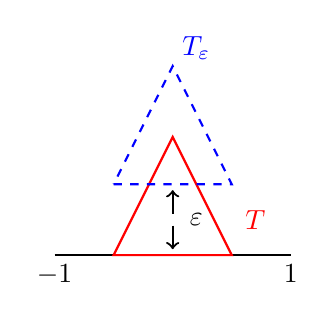
\begin{tikzpicture}[scale=1.5]

		% Draw the real axis segment [-1,1]
		\draw[thick] (-1,0) -- (1,0);
		\draw (-1,0) node[below] {$-1$};
		\draw (1,0) node[below] {$1$};

		% Original triangle T
		\draw[thick, red] (-0.5,0) -- (0.5,0) -- (0,1) -- cycle;
		\node[red] at (.7,.3) {$T$};

		% Shifted triangle T_eps
		\draw[thick, blue, dashed] (-0.5,0.6) -- (0.5,0.6) -- (0,1.6) -- cycle;
		\node[blue] at (.2,1.75) {$T_\varepsilon$};

		% Vertical arrows showing displacement epsilon
		\draw[->, thick] (0,0.35) -- (0,0.55);
		\draw[->, thick] (0,0.25) -- (0,0.05);
		\node at (0.2,0.3) {$\varepsilon$};
	\end{tikzpicture}
	\caption{\small
		The triangle $T$ touches the segment $[-1,1]$ on the real axis.
		Shifting it vertically by $\varepsilon>0$ produces the translated triangle
		$T_\varepsilon = T + i\varepsilon$, which lies entirely in $\mathbb{C}\setminus[-1,1]$.
	}
	\label{fig:tpath}
\end{figure}


\begin{proof}
	We assume $f:\mathbb{C}\to\mathbb{C}$ is continuous on $\mathbb{C}$ and analytic on
	$\mathbb{C}\setminus[-1,1]$.
	By Morera’s theorem, it suffices to prove that
	\[
		\int_T f(z)\,dz = 0
	\]
	for every triangular path $T$ in $\mathbb{C}$.

	\medskip
	\noindent\textbf{Case 1: $T$ and its interior avoid $[-1,1]$.}
	If
	\[
		T \cup \mathrm{Int}(T) \subset \mathbb{C}\setminus[-1,1],
	\]
	then $f$ is analytic in a neighborhood of $T$, and by Cauchy’s theorem,
	\[
		\int_T f(z)\,dz = 0.
	\]

	\medskip
	\noindent\textbf{Case 2: One side of $T$ lies on the segment $[-1,1]$.}

	This is the configuration shown in Figure~\ref{fig:tpath}:
	the base of the triangle lies on $[-1,1]$ while the remaining two sides lie in the upper half–plane.
	Let $T$ denote this triangle.
	For $\varepsilon>0$ define its vertical translate
	\[
		T_\varepsilon = T + i\varepsilon.
	\]
	As illustrated in Figure~\ref{fig:tpath}, when $\varepsilon>0$ is small,
	the entire triangle $T_\varepsilon$ (together with its interior) lies strictly above the real axis and therefore satisfies
	\[
		T_\varepsilon \cup \mathrm{Int}(T_\varepsilon)
		\subset\mathbb{C}\setminus[-1,1].
	\]
	Thus, by Case~1,
	\[
		\int_{T_\varepsilon} f(z)\,dz = 0
		\qquad\text{for all sufficiently small }\varepsilon>0.
	\]

	Let $\gamma:[0,1]\to\mathbb{C}$ parametrize $T$.
	Then
	\[
		\gamma_\varepsilon(t)=\gamma(t)+i\varepsilon
	\]
	parametrizes $T_\varepsilon$, and clearly $\gamma_\varepsilon\to\gamma$
	\emph{uniformly} on $[0,1]$ as $\varepsilon\to 0$.

	Since $f$ is continuous on $\mathbb{C}$, it is uniformly continuous on the compact set
	\[
		K:=\bigcup_{0\le\varepsilon\le\varepsilon_0} T_\varepsilon
	\]
	for some small $\varepsilon_0$.
	Therefore $f(\gamma_\varepsilon(t))$ converges uniformly to $f(\gamma(t))$.
	Hence we may pass the limit inside the integral:
	\[
		\int_T f(z)\,dz
		= \int_0^1 f(\gamma(t))\,\gamma'(t)\,dt
		= \lim_{\varepsilon\to 0}\int_0^1 f(\gamma_\varepsilon(t))\,\gamma_\varepsilon'(t)\,dt
		= \lim_{\varepsilon\to 0} \int_{T_\varepsilon} f(z)\,dz = 0.
	\]

	\medskip
	\noindent\textbf{General case.}

	If $T$ intersects $[-1,1]$ in any other way, we divide $T$ into finitely many smaller triangles by inserting straight segments between the points of intersection with $[-1,1]$. A typical example of such a configuration is illustrated in
	Figure~\ref{fig:spath}.
	Each subtriangle is either of type~1 or type~2.
	Applying the two cases above to each subtriangle and summing the resulting integrals yields
	\[
		\int_T f(z)\,dz = 0.
	\]

	\medskip
	\noindent\textbf{Conclusion.}
	Since $\int_T f\,dz=0$ for every triangular path $T$ and $f$ is continuous on $\mathbb{C}$,
	Morera’s theorem implies that $f$ is analytic on all of $\mathbb{C}$.
	Thus $f$ is entire.
\end{proof}

\begin{figure}[t]
	\centering
	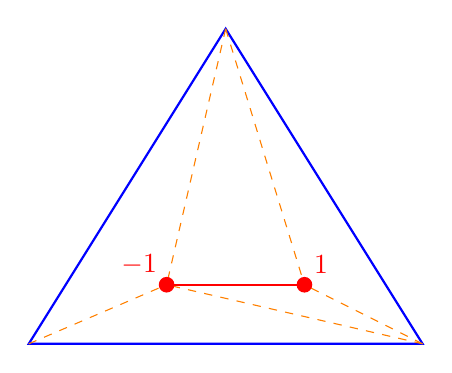
\begin{tikzpicture}[scale=2.5]

		% Coordinates (adjusted to match your sketch)
		\coordinate (d) at (0,1.8);
		\coordinate (e) at (-1,.2);
		\coordinate (c) at (1,0.2);

		\coordinate (b) at (-0.3,0.5);
		\coordinate (a) at (0.4,0.5);

		% Outer triangle (blue)
		\draw[thick, blue] (d) -- (e) -- (c) -- cycle;

		% Subdivision lines (orange)
		\draw[dashed, orange] (d) -- (b);
		\draw[dashed, orange] (d) -- (a);
		\draw[dashed, orange] (e) -- (b);
		\draw[dashed, orange] (c) -- (a);
		\draw[dashed, orange] (c) -- (b);

		% Red connecting segment
		\draw[thick, red] (b) -- (a);

		% Draw points for a, b
		\node[fill=red, circle, inner sep=2pt] at (a) {};
		\node[fill=red, circle, inner sep=2pt] at (b) {};

		% Labels for a, b
		\node[red, right] at (0.4,0.6) {$1$};
		\node[red, left] at (-0.3,0.6) {$-1$};


	\end{tikzpicture}
	\caption{\small
		Subdivision of a triangle by two interior points $1$ and $-1$ and the segment joining them.
	}
	\label{fig:spath}
\end{figure}

\section*{\S6. The homotopic version of Cauchy's Theorem and simple connectivity}
\setexercise{5}
\begin{exercise}
	Evaluate the integral $\displaystyle \int_{\gamma} \frac{dz}{z^{2}+1}$ where $\gamma(\theta) = 2|\cos 2\theta|\, e^{i\theta}$ for $0 \le \theta \le 2\pi$.
\end{exercise}

\begin{proof}
	We are given the curve
	\[
		\gamma(\theta)=2|\cos 2\theta|\,e^{i\theta}, \qquad 0\le \theta\le 2\pi,
	\]
	and we wish to evaluate
	\[
		\int_\gamma \frac{dz}{z^{2}+1}.
	\]

	\textbf{Step 1: Homotope $\gamma$ to the circle $|z|=2$.}
	Define a homotopy
	\[
		H(s,\theta)
		=\big[(1-s)\,2|\cos 2\theta|+2s\big]e^{i\theta},
		\qquad 0\le s\le 1,\ 0\le\theta\le 2\pi.
	\]
	Then $H(0,\theta)=\gamma(\theta)$ and $H(1,\theta)=2e^{i\theta}$.
	We claim $H(s,\theta)\neq \pm i$ for all $(s,\theta)$.
	Indeed, $\pm i$ have modulus $1$, whereas
	\[
		|H(s,\theta)|=(1-s)\,2|\cos 2\theta|+2s\ge 2s\ge 0,
	\]
	and for $\theta=\frac{\pi}{2},\frac{3\pi}{2}$ one has $|H(s,\theta)|=2$.
	Thus $H$ never hits $\pm i$, and therefore gives a homotopy in
	$\mathbb{C}\setminus\{\pm i\}$ from $\gamma$ to the circle
	\[
		\delta(\theta)=2e^{i\theta}.
	\]

	Since $f(z)=\frac{1}{z^{2}+1}$ is analytic on $\mathbb{C}\setminus\{\pm i\}$,
	it follows from homotopy invariance of contour integrals that
	\[
		\int_\gamma \frac{dz}{z^{2}+1}
		=\int_\delta \frac{dz}{z^{2}+1}.
	\]

	\textbf{Step 2: Partial fractions and winding numbers.}
	We write
	\[
		\frac{1}{z^{2}+1}
		=\frac{1}{(z-i)(z+i)}
		=\frac{1}{2i}\left(\frac{1}{z-i}-\frac{1}{z+i}\right).
	\]
	Thus
	\[
		\int_\delta \frac{dz}{z^{2}+1}
		=\frac{1}{2i}
		\left(
		\int_\delta \frac{dz}{z-i}
		-
		\int_\delta \frac{dz}{z+i}
		\right).
	\]

	Now $\delta(\theta)=2e^{i\theta}$ winds once counterclockwise about both
	$i$ and $-i$, since both satisfy $|\,\pm i\,|=1<2$.  Hence
	\[
		n(\delta;i)=1, \qquad n(\delta;-i)=1.
	\]
	By the winding number formula,
	\[
		\int_\delta \frac{dz}{z-i}=2\pi i\cdot n(\delta;i)=2\pi i,
		\qquad
		\int_\delta \frac{dz}{z+i}=2\pi i\cdot n(\delta;-i)=2\pi i.
	\]

	Therefore
	\[
		\int_\delta \frac{dz}{z^{2}+1}
		=\frac{1}{2i}(2\pi i-2\pi i)=0.
	\]

	Hence
	\[
		\int_\gamma \frac{dz}{z^{2}+1}=0.
	\]
\end{proof}


\setexercise{6}
\begin{exercise}
	Let $\gamma(\theta) = \theta e^{i\theta}$ for $0 \le \theta \le 2\pi$ and $\gamma(\theta)= 4\pi - \theta$ for $2\pi \le \theta \le 4\pi$.
	Evaluate $\displaystyle \int_{\gamma} \frac{dz}{z^{2} + \pi^{2}}$.
\end{exercise}

\begin{figure}[h]
	\centering
	\begin{tikzpicture}[scale=0.5]
		% axes
		\draw[->] (-1,0) -- (9,0) node[right] {$\Re z$};
		\draw[->] (0,-7) -- (0,7) node[above] {$\Im z$};

		% mark i pi and -i pi
		\fill (0,3.1416) circle (2pt) node[above right] {$i\pi$};
		\fill (0,-3.1416) circle (2pt) node[below right] {$-i\pi$};

		% spiral: z = theta e^{i\theta}, 0 <= theta <= 2 pi
		\draw[thick, blue, domain=0:6.283, samples=300, variable=\t,
			postaction={decorate},
			decoration={markings, mark=at position 0.25 with {\arrow{>}},
					mark=at position 0.55 with {\arrow{>}},
					mark=at position 0.85 with {\arrow{>}}}]
		plot ({\t*cos(\t r)}, {\t*sin(\t r)});

		% straight return from 2pi to 0
		\draw[thick, blue, postaction={decorate},
			decoration={markings, mark=at position 0.5 with {\arrow{>}}}]
		(6.283,0) -- (0,0);

		% mark 0 and 2 pi
		\fill (0,0) circle (2pt) node[below left] {$0$};
		\fill (6.283,0) circle (2pt) node[below] {$2\pi$};

		% annotations
		\node[blue] at (4,2.5) {$\gamma(\theta)=\theta e^{i\theta}$};
		\node[blue] at (3,-1) {$\gamma(\theta)=4\pi-\theta$};
	\end{tikzpicture}
	\caption{The path $\gamma$: a spiral from $0$ to $2\pi$ followed by a straight line back to $0$.
		The spiral encloses the point $-i\pi$ but not $i\pi$.}
	\label{fig:path}
\end{figure}

\begin{proof}
	The curve $\gamma$ is defined by
	\[
		\gamma(\theta)=
		\begin{cases}
			\theta e^{i\theta}, & 0\le \theta \le 2\pi,     \\[4pt]
			4\pi-\theta,        & 2\pi \le \theta \le 4\pi.
		\end{cases}
	\]
	For $0\le\theta\le 2\pi$ the point $\theta e^{i\theta}$ traces a spiral beginning at $0$,
	making one full revolution around the origin, and reaching the point $2\pi$ on the real axis.
	For $2\pi\le\theta\le 4\pi$ the path travels along the real axis from $2\pi$ back to $0$.
	The resulting curve is shown in Figure~\ref{fig:path}.

	\medskip
	The curve winds once counterclockwise
	around the point $-i\pi$, which lies inside the spiral,
	and does not wind around the point $i\pi$, which lies outside the spiral.
	Thus the winding numbers are
	\[
		n(\gamma;-i\pi)=1,
		\qquad
		n(\gamma;i\pi)=0.
	\]

	We compute the integral
	\[
		\int_\gamma \frac{dz}{z^{2}+\pi^{2}}.
	\]
	Using the partial fraction decomposition
	\[
		\frac{1}{z^{2}+\pi^{2}}
		=\frac{1}{(z-i\pi)(z+i\pi)}
		=\frac{1}{2\pi i} \left( \frac{1}{z-i\pi} - \frac{1}{z+i\pi} \right),
	\]
	we obtain
	\[
		\int_\gamma \frac{dz}{z^{2}+\pi^{2}}
		=
		\frac{1}{2\pi i}
		\left(
		\int_\gamma \frac{dz}{z-i\pi}
		-
		\int_\gamma \frac{dz}{z+i\pi}
		\right).
	\]

	By the winding number formula,
	\[
		\int_\gamma \frac{dz}{z-a}
		=
		2\pi i\, n(\gamma;a),
	\]
	so using the winding numbers read off from Figure~\ref{fig:path},
	\[
		\int_\gamma \frac{dz}{z-i\pi}
		=2\pi i\,n(\gamma;i\pi)=0,
		\qquad
		\int_\gamma \frac{dz}{z+i\pi}
		=2\pi i\,n(\gamma;-i\pi)=2\pi i.
	\]

	Substituting these into the previous expression gives
	\[
		\int_\gamma \frac{dz}{z^{2}+\pi^{2}}
		=
		\frac{1}{2\pi i}(0-2\pi i)
		= -1.
	\]
\end{proof}


\setexercise{7}
\begin{exercise}
	Let
	\(
	f(z) = \big[(z - \tfrac{1}{2} - i)(z - 1 - \tfrac{3}{2}i)(z - 1 - i)(z - \tfrac{3}{2} - i)\big]^{-1}
	\)
	and let $\gamma$ be the polygon $[0,\, 2,\, 2+2i,\, 2i,\, 0]$.
	Find $\displaystyle \int_{\gamma} f$.
\end{exercise}

\begin{proof}
	Let
	\[
		f(z)=\frac{1}{
			(z-z_1)(z-z_2)(z-z_3)(z-z_4)},
	\]
	where
	\[
		z_1=\tfrac12+i,\qquad
		z_2=1+\tfrac32 i,\qquad
		z_3=1+i,\qquad
		z_4=\tfrac32+i.
	\]
	These are four distinct points, so the partial fraction expansion has the form
	\[
		f(z)=
		\sum_{k=1}^4
		\frac{A_k}{z-z_k},
	\]
	where
	\[
		A_k=\frac{1}{
			\displaystyle \prod_{j\ne k}(z_k-z_j)}.
	\]

	Thus
	\[
		\int_\gamma f(z)\,dz
		=\sum_{k=1}^4 A_k
		\int_\gamma \frac{dz}{z-z_k}.
	\]

	The path
	\[
		\gamma=[0,\,2,\,2+2i,\,2i,\,0]
	\]
	is the positively oriented boundary of the square
	\[
		0<\Re z<2,\qquad 0<\Im z<2.
	\]
	A simple check of real and imaginary parts shows that all four points
	\(z_1,z_2,z_3,z_4\) lie inside this square.
	Therefore
	\[
		n(\gamma;z_k)=1
		\qquad\text{for }k=1,2,3,4,
	\]
	and hence
	\[
		\int_\gamma \frac{dz}{z-z_k}
		=2\pi i.
	\]

	Therefore
	\[
		\int_\gamma f(z)\,dz
		=\sum_{k=1}^4 A_k \cdot 2\pi i
		=
		2\pi i \sum_{k=1}^4 A_k.
	\]

	It remains to compute the four coefficients \(A_k\).  A direct computation gives
	\[
		A_1=-2+2i,\qquad
		A_2=-4i,\qquad
		A_3=-8i,\qquad
		A_4=2+2i.
	\]

	Adding them,
	\[
		A_1+A_2+A_3+A_4
		=(-2+2)+(2i-4i-8i+2i)
		=-8i.
	\]

	Thus
	\[
		\int_\gamma f(z)\,dz
		=2\pi i\,(-8i)
		=16\pi.
	\]
\end{proof}


\setexercise{10}
\begin{exercise}
	Find all possible values of $\displaystyle \int_{\gamma} \frac{dz}{1 + z^{2}}$ where $\gamma$ is any closed rectifiable curve.
\end{exercise}

\begin{proof}
	We use the partial fraction decomposition
	\[
		\frac{1}{1+z^{2}}
		=\frac{1}{(z-i)(z+i)}
		=\frac{1}{2i}\left(\frac{1}{z-i}-\frac{1}{z+i}\right).
	\]
	For any closed rectifiable curve $\gamma$ and any $a\in\mathbb{C}$, we have
	\[
		\int_\gamma \frac{dz}{z-a}
		= 2\pi i\, n(\gamma;a),
	\]
	where $n(\gamma;a)$ is the winding number of $\gamma$ about $a$.
	Therefore
	\[
		\int_\gamma \frac{dz}{1+z^{2}}
		=\frac{1}{2i}
		\left(2\pi i\, n(\gamma;i) - 2\pi i\, n(\gamma;-i)\right)
		=\pi\bigl(n(\gamma;i)-n(\gamma;-i)\bigr).
	\]

	Since $n(\gamma;i)$ and $n(\gamma;-i)$ may be any integers (positive, negative, or zero)
	depending on how the curve winds around $i$ and $-i$, the integral may take any value of the form
	\[
		\{\pi k : k\in\mathbb{Z}\}.
	\]
\end{proof}
\section*{\S7. Counting zeros; the Open Mapping Theorem}
\setexercise{4}
\begin{exercise}
	Suppose that $f : G \to \mathbb{C}$ is analytic and one--one; show that $f'(z) \neq 0$ for any $z$ in $G$.
\end{exercise}


\begin{proof}
	Let $f : G \to \mathbb{C}$ be analytic and one--one, and fix a point
	$a \in G$.  We show that $f'(a) \neq 0$.
	Suppose for contradiction that $f'(a)=0$.
	Then $f(z)-f(a)$ has a zero at $z=a$ of multiplicity $m \ge 2$.
	By Theorem~7.4, there exist $\varepsilon>0$ and $\delta>0$ such that
	whenever $0<|\zeta - f(a)| < \delta$, the equation
	\[
		f(z)=\zeta
	\]
	has \emph{exactly $m$ distinct solutions} in the disk $B(a;\varepsilon)$.
	Since $m\ge 2$, every $\zeta$ sufficiently close to $f(a)$ is taken at
	least twice by $f$.
	This contradicts the assumption that $f$ is one--one on~$G$.
	Therefore our assumption was impossible, and we must have $f'(a) \neq 0$.
	As $a$ was arbitrary, it follows that
	\[
		f'(z) \neq 0 \qquad \text{for all } z \in G.
	\]
\end{proof}

\end{document}
